\documentclass{jknotes}
\usepackage{joshkirklin}

\institution{Cambridge Part III Maths}
\title{Cosmology}
\lecturer{James Fergusson and David Marsh}
\notetaker{Josh Kirklin}
\date{Michaelmas 2015}

\begin{document}

\maketitle
\suggestionsspiel

\tableofcontents

\section{Geometry and Dynamics}
\subsection{Metric}
To star with, we will make three assumptions:
\begin{enumerate}
    \item The universe is isotropic (i.e.\ the same in all directions and rotation invariant).
    \item The universe is homogeneous (i.e.\ the same in all locations and translation invariant).
    \item General relativity holds on the scale of the universe.
\end{enumerate}

There is strong evidence for 1 and 2 from the cosmic microwave background (CMB). On solar system scales, there is strong evidence for 3, and also strong evidence on larger scales provided we assume that dark energy and dark matter exist.

1,2 and 3 together force the metric to take the form
\begin{equation}
    \dd{s}^2 = g_{\mu\nu}\dd{x^\mu}\dd{x^\nu} = -\dd{t}^2+\dd{l}^2,
\end{equation}
where \(\dd{l}^2\) is a constant curvature 3-metric, which can only have one of three forms:
\begin{itemize}
    \item Constant positive curvature --- spherical --- \(\dd{l}^2 = \dd{\vb{x}}^2 + \dd{u}^2\), \(\vb{x}^2+u^2=a^2\)
    \item Zero curvature --- Euclidean --- \(\dd{l}^2=\dd{\vb{x}}^2\)
    \item Constant negative curvature --- hyperbolic --- \(\dd{l}^2 = \dd{\vb{x}}^2 - \dd{u}^2\), \(\vb{x}^2-u^2=a^2\)
\end{itemize}
where \(\vb{x}\) and \(u\) are some coordinates. Eliminating \(u\), and taking \(\vb{x}\to a\vb{x}, u\to au\), we have
\begin{align}
    \dd{l}^2 &= a^2(\dd{x}^2\pm\dd{u}^2) \\
             &= a^2\left(\dd{\vb{x}}^2 + k\frac{(\vb{x}\vdot\dd{\vb{x}})^2}{1-k\vb{x}^2}\right) 
\end{align}
where \(k= 1\) for spherical space, \(0\) for Euclidean space, and \(-1\) for hyperbolic space. Writing this in spherical coordinates and substituing back into the 4-metric, we obtain
\begin{equation}
    \dd{s}^2 = -\dd{t}^2 + a^2\left(\frac{\dd{r}^2}{1-kr^2}+r^2\dd{\Omega}\right).
\end{equation}
This is the Friedmann-Lema\^itre-Robertson-Walker (FLRW) metric. \(a\) is called the \emph{scale factor}, and in general depends on time.

This metric is invariant under a rescaling \(a\to \lambda a, r\to \frac{r}{\lambda}, k\to \lambda^2 k\). We usually use this to set \(a=1\) today (\(a_0=a(t_0)=1\)).

\(r\) is called a \emph{comoving} coordinate. The associated physical coordinate is \(r_{\text{ph}}=ar\). In a similar way, the physical curvature is \(k_{\text{ph}}=\frac{k}{a^2}\). The physical velocity of an object in FLRW space is given by
\begin{equation}
    v_{\text{ph}} = \dv{r_{\text{ph}}}{t} = a\dv{r}{t} + \dv{a}{t}r = v_{\text{pec}} + Hr_{\text{ph}},
\end{equation}
where \(H=\frac{\dot{a}}{a}\) is \emph{Hubble's ``constant''}, and \(v_{\text{pec}}=a\dv{r}{t}\) is the \emph{peculiar velocity}. We call the \(Hr_{\text{ph}}\) contribution the \emph{Hubble flow}.

Often we will use conformal time \(\tau\), defined by \(\dd{t}=a\dd{\tau}\), or equivalently \(\tau = \int\frac{\dd{t}}{a}\). The metric then takes the form
\begin{equation}
    \dd{s}^2 = a^2\Big(\underbrace{-\dd{\tau}^2+\frac{\dd{r}^2}{1-kr^2}+r^2\dd{\Omega}^2}_{\text{static}}\Big).
\end{equation}

Sometimes we prefer to use the coordinate \(\chi\) instead of \(r\), where \(\chi = \int\frac{\dd{r}}{\sqrt{1-kr^2}}\). With \(\chi\) and \(\tau\), the metric takes the form
\begin{equation}
    \dd{s}^2 = a^2\Big(-\dd{\tau}^2 + \dd{\chi}^2 + 
        \begin{Bmatrix}
            \sin^2\chi & S^3 \\
            \chi^2 & E^3 \\
            \sinh^2\chi & H^3
        \end{Bmatrix}
    \dd{\Omega}^2\Big).
\end{equation}

\subsection{Kinematics}
Suppose gravity is the only force in the universe. Then test particles move on geodesics. A particle of mass \(m\) has 4-velocity \(U^\mu=\dv{x^\mu}{s}\), and its motion is defined by the geodesic equation
\begin{equation}
    \dv{U^\mu}{s} + \Gamma^\mu_{\alpha\beta} U^\alpha U^\beta = 0,
\end{equation}
where
\begin{equation}
    \Gamma^\mu_{\alpha\beta} = \frac{1}{2}g^{\mu\lambda}(g_{\beta\lambda,\alpha} + g_{\alpha\lambda,\beta} - g_{\alpha\beta,\lambda}).
\end{equation}
Using \(\dv{U^\mu}{s} = \dv{x^\alpha}{s}\pdv{U^\mu}{x^\alpha} = U^\alpha\pdv{U^\mu}{x^\alpha}\), we then have
\begin{equation}
    U^\alpha\left(\pdv{U^\mu}{x^\alpha} + \Gamma^\mu_{\alpha\beta}U^\beta\right) = U^\alpha\nabla_\alpha U^\mu = 0,
\end{equation}
where \(\nabla\) is the covariant derivative associated with \(\Gamma\). Writing this in terms of the 4-momentum \(P^\alpha=m U^\alpha\), we have
\begin{equation}
    P^\alpha \pdv{P^\mu}{x^\alpha} = - \Gamma^\mu_{\alpha\beta}P^\alpha P^\beta,
\end{equation}
and this works for massless particles too.

Exercise: show that for FLRW (\(g_{00}=-1\), \(g_{0i}=0\), \(g_{ij}=a^2\gamma_{ij}\)) we have
\begin{align}
    \Gamma^\mu_{00} &= \Gamma^0_{0\beta} = 0, \\
    \Gamma^0_{ij} &= a\dot{a}\gamma_{ij}, \\
    \Gamma^i_{0j} &= \frac{\dot{a}}{a}\delta_j^i, \\
    \Gamma^i_{jk} &= \Gamma^{(3) i}_{jk} = 0 \; \text{in \(E^3\)}.
\end{align}

Homogeneity implies that \(\partial_i P^\mu=0\), so we have
\begin{equation}
    P^0\dv{P\mu}{t} = -\Gamma^\mu_{\alpha\beta}P^\alpha P^\beta = (-2\Gamma^\mu_{0j}p^0 + \Gamma^\mu_{ij}p^i)p^j.
\end{equation}
This implies two things:
\begin{itemize}
    \item Suppose \(P^i=0\). Then \(\dv{P^i}{t}=0\), i.e.\ particles at rest remain so.
    \item Setting \(\mu=0\), we have \(E\dv{E}{t}=-\frac{\dot{a}}{a}p^2\), where \(E\) is the energy of the particle and \(p\) is it's physical 3-momentum (so \(p^2 = a^2\gamma_{ij}P^iP^j\)). Using \(m^2=-E^2+p^2\), we have \(E\dd{E}=p\dd{p}\), so \(\frac{\dot{p}}{p}=\frac{\dot{a}}{a}\), and hence \(p(t)\propto\frac{1}{a(t)}\). Suppose we are in an expanding universe. Then for massless particles, we have \(E=|p|\propto\frac{1}{\alpha}\), so energies decay, and for massive particles \(p = \frac{mv}{\sqrt{1-v^2}}\propto \frac{1}{\alpha}\), so peculiar veclocities decay.
\end{itemize}

\subsection{Redshift}
A photon's wavelength is given by \(\lambda = \frac{h}{|p|}\), so we have \(\lambda \propto a\). Consider light emitted at time \(t_1\) with wavelength \(\lambda_1\). We observe the light at time \(t_0\) with wavelength \(\lambda_0\). Then \(\lambda_0=\frac{a_0}{a_1}\lambda_1 > \lambda_1\). We define the \emph{redshift} in the light by
\begin{equation}
    Z = \frac{\lambda_0-\lambda_1}{\lambda_1}.
\end{equation}
If we set \(a_0=1\), then we have \(1+z=\frac{1}{\alpha}\). For nearby sources, \(z\) and \(t_0-t_1\) are both small, so we can do a series expansion to find
\begin{equation}
    1 - z + \dots = \frac{1}{1+z} = a(t) = 1 + (t_1-t_0)H_0 + \frac{1}{2}H_0^2q_0(t_1-t_0)^2+\dots,
\end{equation}
where \(q\) is the so-called \emph{deceleration parameter}. Writing \(d=t_0-t_1\), we have
\begin{equation}
    z = H_0d + O(H_0^2(t_1-t_0)^2).
\end{equation}
This is ``Hubble's law'', and it empirically remains valid for \(z\) up to about \(0.5\).
\begin{figure}[H]
    \centering
    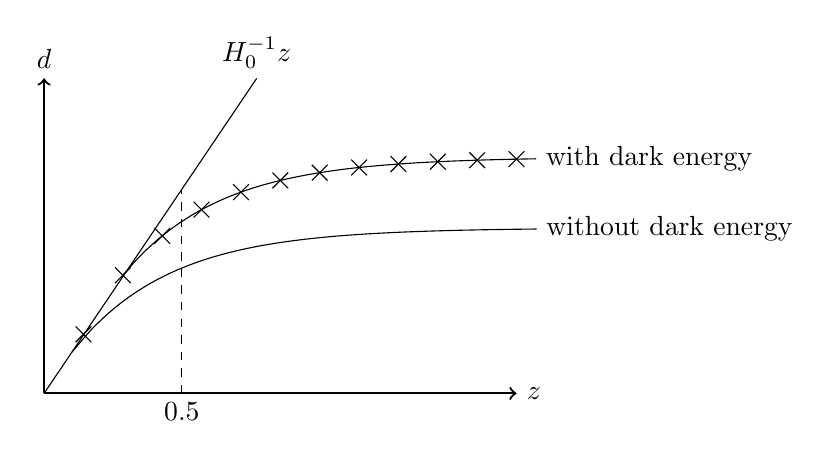
\begin{tikzpicture}
        \draw[thick,->] (0,0) -- (6,0) node[right] {\(z\)};
        \draw[thick,->] (0,0) -- (0,4) node[above] {\(d\)};
        \foreach \x in {1,2,3,4,5,6,7,8,9,10,11,12} {
            \begin{scope}[shift={(\x/2,3-1.5^(3-\x))},scale=0.1]
                \draw (-1,-1) -- (1,1);
                \draw (-1,1) -- (1,-1);
            \end{scope}
        }
        \draw (0,0) -- (2.7,4) node[above] {\(H_0^{-1}z\)};
        \draw[domain=2:12.5,smooth,variable=\x] plot({\x/2},{3-1.5^(3-\x)}) node[right] {with dark energy};
        \draw[domain=1:12.8,smooth,variable=\x] plot({\x/2-0.145},{(3-1.5^(3-\x))*0.7}) node[right] {without dark energy};
        \draw[dashed] (1.75,0) node[below] {\(0.5\)} -- (1.75,{1.75*4/2.7});
    \end{tikzpicture}
\end{figure}
The best current measurements give \(H_0=100h\,\si{\kilo\metre\second^{-1}\mega\parsec^{-1}}\), where \(h=0.67\pm0.01\).

\subsection{Dynamics}
The evolution of the scale factor \(a(t)\) is determined by the Einstein equations \(G_{\mu\nu} = 8\pi G T_{\mu\nu}\), where we are defining the energy-momentum tensor to include the possibility of a cosmological constant term. The components of \(T\) describe the properties of matter in the universe in the following way:
\begin{equation}
    T_{\mu\nu} =
    \begin{pmatrix}
        T_{00} & T_{0j} \\
        T_{i0} & T_{ij}
    \end{pmatrix} 
    =
    \begin{pmatrix}
        \text{energy density} & \text{energy current} \\
        \text{momentum density} & \text{stress tensor}
    \end{pmatrix}
\end{equation}

Suppose a particular species of matter has number current \(N_\mu=(N_0,N_i)\), where \(N_0\) is number density, and \(N_i\) is number flux. Then to a comoving observer (i.e.\ one with vanishing peculiar velocity), homogeneity and isotropy imply \(N_i=0\). We define \(n(t)\) to be the value of \(N_0\) in this frame. We also have \(T_{0i}=T_{i0}\), and we define the density \(\rho\) and pressure \(P\) of matter by
\begin{equation}
    T_{00} = -\rho(t) \qq{and} T_{ij} = P(t)g_{ij}.
\end{equation}
To a general observer, we have \(N_\mu = n U_\mu\) and \(T_{\mu\nu} = (\rho+P)U_\mu U_\nu + Pg_{\mu\nu}\). 

There are conversation laws associated with \(N\) and \(T\). We have
\begin{equation}
    \nabla_\mu N^\mu = 0 \implies \partial_\mu N^\mu + \Gamma^\mu_{\mu\lambda} N^\lambda = 0 \implies \frac{\dot{n}}{n} = -3\frac{\dot{a}}{a} \implies n \propto a^{-3}.
\end{equation}
Also
\begin{equation}
    \nabla_\mu T^\mu_\nu = \partial_\mu T^\mu_\nu + \Gamma^\mu_{\mu\lambda}T^\lambda_\nu - \gamma^\lambda_{\mu\nu}T^\mu_\nu = 0 \implies \dot{\rho} + 3\frac{\dot{a}}{a}(\rho+P)=0.
\end{equation}
Note that this gives
\begin{equation}
    \dv{(\rho a^3)}{t} = -P\dv{(a^3)}{t},
\end{equation}
which we can identify with the first law of thermodynamics \(\dd{U}=-P\dd{V}\).

Suppose now that \(P\propto\rho\), and define \(w = \frac{P}{\rho}\). Then we have
\begin{equation}
    \frac{\dot{\rho}}{\rho} = -3(1+w)\frac{\dot{a}}{a} \implies \rho \propto a^{-3(1+w)}.
\end{equation}

Most matter that we consider will have \(P\propto\rho\). The following is a cosmic inventory of such matter:
\begin{table}[H]
    \centering
    \begin{tabular}{cclcc}
        Matter & (\(m\)) & 
        $\Bigg\{$
        \begin{tabular}{lc}
            CDM & (\(c\)) \\
            Baryons & (\(b\))
        \end{tabular} &
        \(w=0\) & \(\rho\propto a^{-3}\) \\
        Radiation & (\(r\)) & 
        $\Bigg\{$
        \begin{tabular}{lc}
            Photons & (\(\gamma\)) \\
            Neutrons & (\(\nu\)) \\
            Gravitons & (\(g\))
        \end{tabular} &
        \(w=\frac{1}{3}\) & \(\rho\propto a^{-4}\) \\
        Dark energy & (\(\Lambda\)) & 
        $\Bigg\{$
        \begin{tabular}{l}
            Vacuum energy \\
            Modified gravity \\
            Cosmological constant \\
            ??????????
        \end{tabular} &
        \(w=-1\) & \(\rho\) constant
    \end{tabular}
\end{table}

Now lets deal with the curvature part of the Einstein equations. We have \(G_{\mu\nu} = R_{\mu\nu} - \frac{1}{2}g_{\mu\nu}R\), where
\begin{equation}
    R_{\mu\nu}=\partial_\lambda\Gamma^\lambda_{\mu\nu} - \partial_\nu\Gamma^\lambda_{\mu\lambda} + \Gamma^\lambda_{\lambda\rho}\Gamma^\rho_{\mu\nu} - \Gamma^\rho_{\mu\lambda}\Gamma^\Lambda_{\nu\rho} \qq{and} R = g^{\mu\nu}R_{\mu\nu}.
\end{equation}
Exercise: show that
\begin{equation}
    R_{00} = -3\frac{\ddot{a}}{a},\quad R_{0i}=0,\quad R_{ij} = \left(-\frac{\ddot{a}}{a} + 2\left(\frac{\dot{a}}{a}\right)^2 + 2\frac{k}{a^2}\right)g_{ij},
\end{equation}
and
\begin{equation}
    G_0^0 = -3\left[\left(\frac{\dot{a}}{a}\right)^2 + \frac{k}{a^2}\right],\quad G^i_j = -\left(2\frac{\ddot{a}}{a} + \left(\frac{\dot{a}}{a}\right)^2 + \frac{k}{a^2}\right)\delta_j^i.
\end{equation}
Therefore the Einstein equations are reduced to
\begin{equation}
    3\left[\left(\frac{\dot{a}}{a}\right)^2+\frac{k}{a^2}\right] = 8\pi G\rho \qq{and} 2\frac{\ddot{a}}{a} + \left(\frac{\dot{a}}{a}\right)^2 + \frac{k}{a^2} = -8\pi GP.
\end{equation}
These rearrange to the \emph{Friedmann equations}:
\begin{align}
    \left(\frac{\dot{a}}{a}\right)^2 &= \frac{8\pi G\rho}{3} - \frac{k}{a^2} \\
    \frac{\ddot{a}}{a} &= -\frac{4\pi G}{3}(\rho + 3P)
\end{align}
Given any two of the Friedmann equations and the conservation equation \(\dot{\rho} = -3\frac{\dot{a}}{a}(\rho+P)\), we can derive the third.

The \emph{critical density} is defined by the density required in order to set \(k=0\). Using the first Friedmann equation, we have
\begin{equation}
    \rho_{\text{crit}} = \frac{3H^2}{8\pi G} \approx \SI{8e-26}{\gram\,\centi\metre^{-3}}\;\text{today}.
\end{equation}

We then define the \emph{density parameter} of a species of matter \(X\) by \(\Omega_X = \frac{\rho_X}{\rho_{\text{crit}}}\). In particular, we have
\begin{align}
    \Omega_r &= \Omega_{r,0} \frac{1}{a^4} \\
    \Omega_m &= \Omega_{m,0} \frac{1}{a^3} \\
    \Omega_\Lambda &= \Omega_{\Lambda,0}.
\end{align}
If we treat the curvature term in the first Friedmann equation as being on the same footing as the density term, we can also define 
\begin{equation}
    \Omega_k = -\frac{k}{(a_0H_0)^2}.
\end{equation}

Writing the Friedmann equations in terms of the density parameters, we have
\begin{align}
    \dot{a}^2 &= H_0^2\left(\frac{\Omega_{r,0}}{a^2} + \frac{\Omega_{m,0}}{a} + \Omega_{\Lambda,0}a^2\right) - k, \\
    \ddot{a} &= -H_0^2\left(\frac{\Omega_{r,0}}{a^3} + \frac{\Omega_{m,0}}{2a^2} - \Omega_{\Lambda,0}a\right).
\end{align}

Note that depending on the values of the density parameters, scale factor and curvature, there is a region where we would have \(\dot{a}^2<0\), which is impossible. We can draw the trajectories of \(a\) for given values of \(k\). First we ignore \(\Lambda\).

\begin{figure}[H]
    \centering
    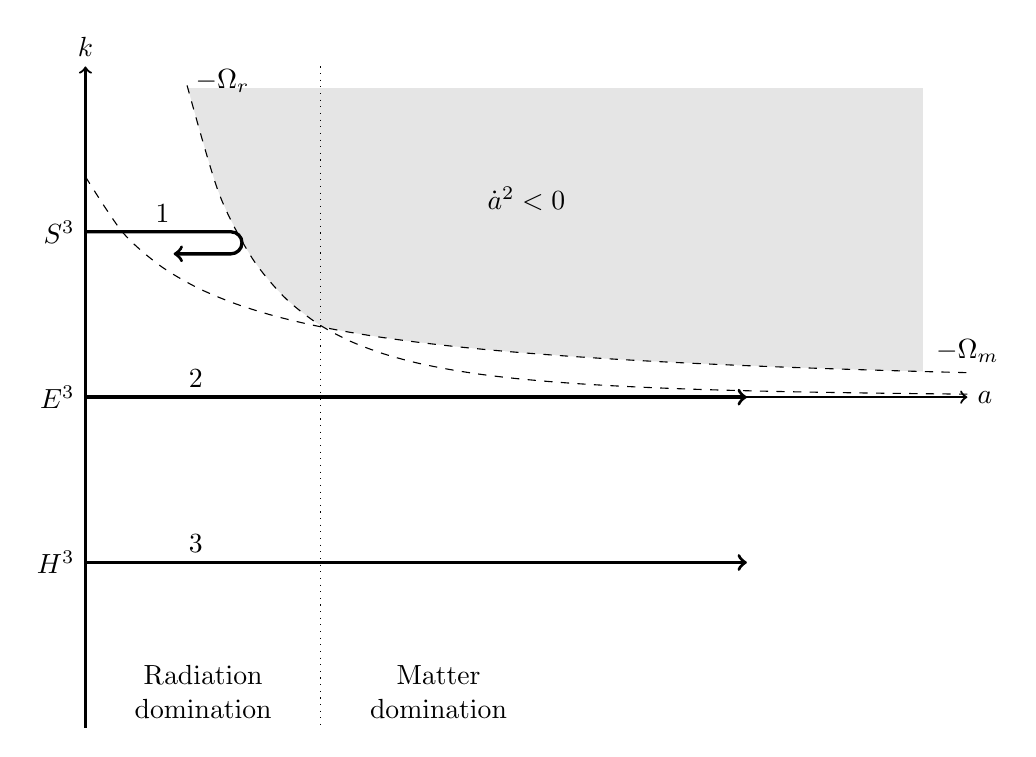
\begin{tikzpicture}[scale=1.4]
        \fill[gray!20] (0,0) rectangle (7.6,2.8);
        \fill[white,domain=0:8,smooth,variable=\x] (0,0) -- plot({\x},{2*(\x+1)^(-1)}) -- (8,0);
        \fill[white,domain=8:0.91,smooth,variable=\x] (0,0) -- plot({\x},{20*(\x+1)^(-3)}) -- (0,3);

        \draw[thick,->] (0,0) -- (8,0) node[right] {\(a\)};
        \draw[thick,->] (0,-3) -- (0,3) node[above] {\(k\)};
        \draw[dashed,domain=0:8,smooth,variable=\x] plot({\x},{2*(\x+1)^(-1)}) node[above] {\(-\Omega_m\)};
        \draw[dashed,domain=8:0.91,smooth,variable=\x] plot({\x},{20*(\x+1)^(-3)}) node[right] {\(-\Omega_r\)};
        \node at (4,1.8) {\(\dot{a}^2<0\)};
        \draw[dotted] (2.135,3) -- (2.135,-3);
        \node[above,align=center] at (1.0675,-3) {Radiation\\domination};
        \node[above,align=center] at (3.2025,-3) {Matter\\domination};

        \draw[very thick,->] (0,-1.5) node[left] {\(H^3\)} -- (6,-1.5);
        \draw[very thick,->] (0,0) node[left] {\(E^3\)} -- (6,0);
        \draw[very thick,->] (0,1.5) node[left] {\(S^3\)} -- (1.32,1.5) arc (90:-90:0.1) -- (0.8,1.3);

        \node[above] at (0.7,1.5) {\(1\)};
        \node[above] at (1,0) {\(2\)};
        \node[above] at (1,-1.5) {\(3\)};
    \end{tikzpicture}
\end{figure}
There are three types of trajectory:
\begin{enumerate}
    \item \(S^3\), \(k>0\), the universe expands then collapses (closed).
    \item \(E^3\), \(k=0\), the universe expands forever, but \(\dot{a}\to0\) as \(t\to0\) (flat).
    \item \(H^3\), \(k<0\), the universe expands forever, and \(\dot{a}\not\to0\) (open).
\end{enumerate}
All trajectories have \(\ddot{a}<0\).

Now include \(\Lambda\). We add a new line to the diagram, reducing the size of the inaccessible region:
\begin{figure}[H]
    \centering
    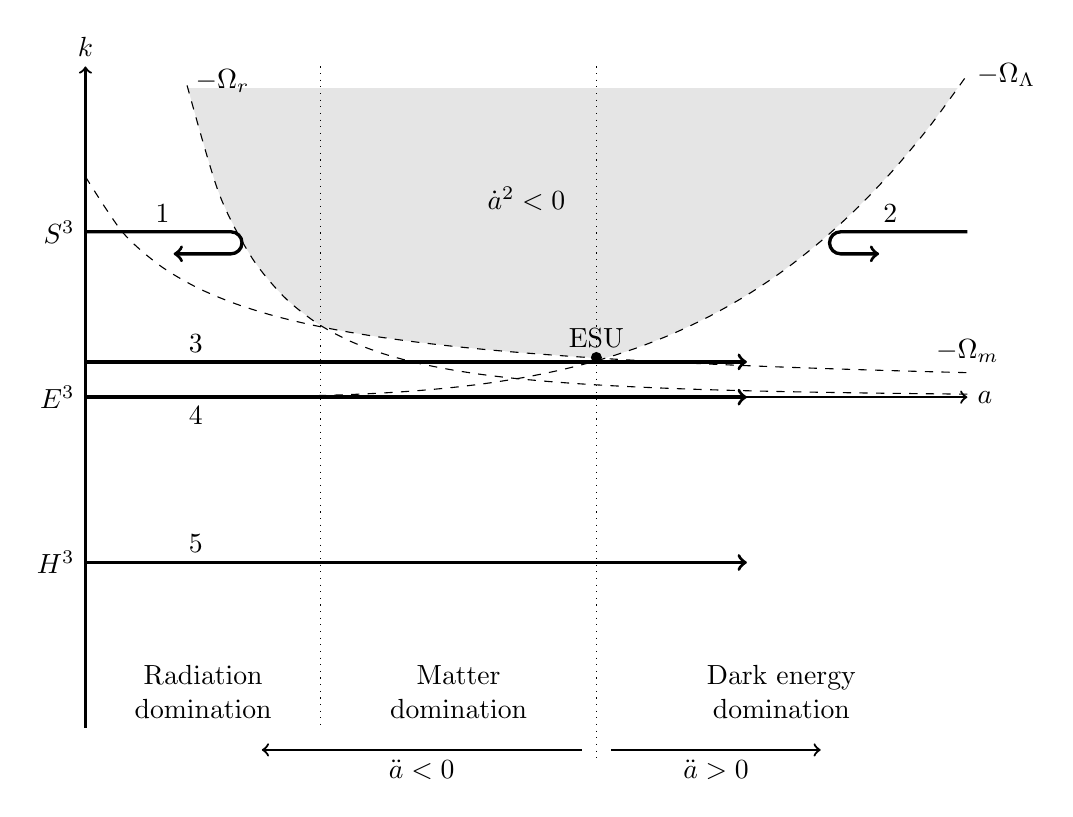
\begin{tikzpicture}[scale=1.4]
        \fill[gray!20] (0,0) rectangle (8,2.8);
        \fill[white,domain=0:8,smooth,variable=\x] (0,0) -- plot({\x},{2*(\x+1)^(-1)}) -- (8,0);
        \fill[white,domain=8:0.91,smooth,variable=\x] (0,0) -- plot({\x},{20*(\x+1)^(-3)}) -- (0,3);
        \fill[white,domain=0:8,smooth,variable=\x] (0,0) -- plot({\x},{(\x^4)/1400}) -- (8,0);

        \draw[thick,->] (0,0) -- (8,0) node[right] {\(a\)};
        \draw[thick,->] (0,-3) -- (0,3) node[above] {\(k\)};
        \draw[dashed,domain=0:8,smooth,variable=\x] plot({\x},{2*(\x+1)^(-1)}) node[above] {\(-\Omega_m\)};
        \draw[dashed,domain=8:0.91,smooth,variable=\x] plot({\x},{20*(\x+1)^(-3)}) node[right] {\(-\Omega_r\)};
        \draw[dashed,domain=0:8,smooth,variable=\x] plot({\x},{(\x^4)/1400}) node[right] {\(-\Omega_\Lambda\)};
        \node at (4,1.8) {\(\dot{a}^2<0\)};
        \draw[dotted] (2.135,3) -- (2.135,-3);
        \draw[dotted] (4.635,3) -- (4.635,-3.3);
        \node[above,align=center] at (1.0675,-3) {Radiation\\domination};
        \node[above,align=center] at (3.385,-3) {Matter\\domination};
        \node[above,align=center] at (6.3125,-3) {Dark energy\\domination};

        \draw[very thick,->] (0,-1.5) node[left] {\(H^3\)} -- (6,-1.5);
        \draw[very thick,->] (0,0) node[left] {\(E^3\)} -- (6,0);
        \draw[very thick,->] (0,0.32) -- (6,0.32);
        \draw[very thick,->] (0,1.5) node[left] {\(S^3\)} -- (1.32,1.5) arc (90:-90:0.1) -- (0.8,1.3);
        \draw[very thick,->] (8,1.5) -- (6.85,1.5) arc (90:270:0.1) -- (7.2,1.3);

        \node[above] at (0.7,1.5) {\(1\)};
        \node[above] at (7.3,1.5) {\(2\)};
        \node[above] at (1,0.32) {\(3\)};
        \node[below] at (1,0) {\(4\)};
        \node[above] at (1,-1.5) {\(5\)};

        \fill (4.635,0.36) circle (0.05) node[above] {ESU};

        \draw[->,thick] (4.5,-3.2) -- (1.6,-3.2) node[midway,below] {\(\ddot{a}<0\)};
        \draw[->,thick] (4.77,-3.2) -- (6.67,-3.2) node[midway,below] {\(\ddot{a}>0\)};
    \end{tikzpicture}
\end{figure}
There are now five scenarios:
\begin{enumerate}
    \item \(S^3\), expansion then collapse (closed).
    \item \(S^3\), collapse then expansion (bouncing).
    \item \(S^3\), expansion, then stall, then expansion (loitering).
    \item \(E^3\), expansion with \(\ddot{a}<0\) then \(\ddot{a}>0\).
    \item \(H^3\), expansion with \(\ddot{a}<0\) then \(\ddot{a}>0\).
\end{enumerate}
We also have the Einstein static universe (ESU), with constant \(a\). 

It can be shown that the ESU is unstable, so we are forced to have a dynamic universe. Also, in order for the universe to have formed structure, it must have had a period of matter domination. Thus we see that the trajectory the universe takes must have had \(a=0\) at some point --- this is the Big Bang.

Observations from the CMB, supernovae, and BAO (Baryon Acoustic Observations) provide the following values:
\begin{equation}
    \begin{matrix}
        \Omega_m = 0.32,\\
        \Omega_b=0.05,\\
        \Omega_c=0.27,\\
        \Omega_\gamma = 10^{-4},\\
        0.001 < \Omega_\nu < 0.02,\\
        |\Omega_k| \le 0.01.
    \end{matrix}
\end{equation}
From now on we will assume \(k=0\).

For the majority of our history, the universe has at any one time been dominated by a single component, so we can take
\begin{equation}
    \left(\frac{\dot{a}}{a}\right)^2 = H_0^2\Omega a^{-3(1+w)}.
\end{equation}
This leads to the following solutions for the scale factor:
\begin{equation}
    a(t) \sim
    \begin{cases}
        t^{\frac{1}{2}} \\
        t^{\frac{2}{3}} \\
        e^{H_0 t}
    \end{cases},\quad
    a(\tau) \sim
    \begin{cases}
        \tau & \text{radiation domination} \\
        \tau^2 & \text{matter domination} \\
        -\frac{1}{\tau} & \text{dark energy domination}
    \end{cases}
\end{equation}
Note that in the final case \(\tau = \int\frac{\dd{t}}{a}\) is negative.

\section{Inflation}
The Big Bang scenario has some notable successes. For example, it predicts the Cosmic Microwave Background (CMB) at about 100,000 years after the Big Bang (BB), and Big Bang Nucleosynthesis correctly predicts the abundancies of the light elements. However, BB has severe problems with initial conditions. These include:
\begin{description}
    \item[Flatness problem:] During matter/radiation domination, deviations from \(k=0\) grow. Since \(k\approx 0\) today, this would imply that \(k\) is extremely fine tuned to be \(|k| \ll\!\!\ll 1\) in the early universe.
    \item[Relics:] Most grand unified theories predict the production of so-called ``relic'' particles (e.g.\ topological defects), and these are not observed.
    \item[Horizon problem:] We observe the CMB to be uniform to 1 part in \(10^5\), but regions in opposite directions are not causally connected.
\end{description}
In this section we will try to solve these problems.

\subsection{Horizon Problem}
First we must define the particle horizon. Considering only radial motion, the FLRW metric in conformal time is given by \(\dd{s}^2 = a^2(\tau)(-\dd{\tau}^2+\dd{\chi}^2)\), where \(\chi = r_{\text{ph}}/a\) is comoving distance. Photons travel on geodesics with \(\dd{s}=0\), so we have \(\Delta\chi = \pm \Delta\tau\), i.e.\ photons travel in straight lines.
\begin{figure}[H]
    \centering
    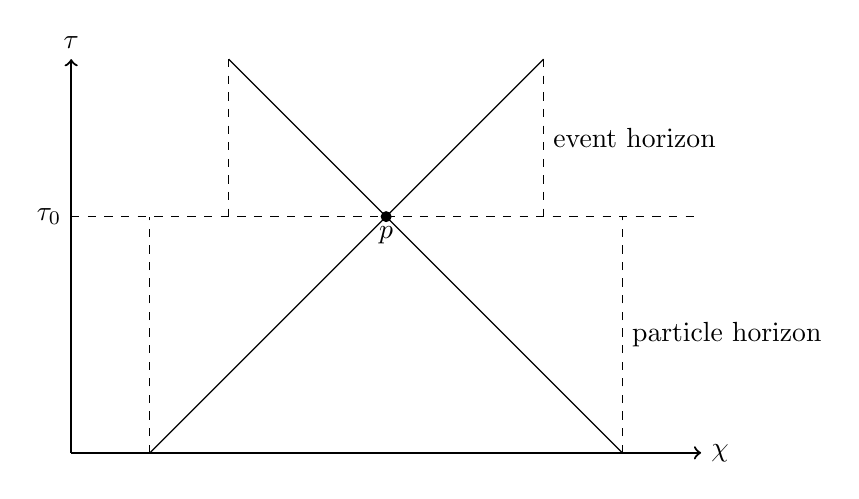
\begin{tikzpicture}
        \draw[thick,->] (0,0) -- (8,0) node[right] {\(\chi\)};
        \draw[thick,->] (0,0) -- (0,5) node[above] {\(\tau\)};
        \draw[dashed] (0,3) node[left] {\(\tau_0\)} -- (8,3);
        \fill (4,3) circle (0.07) node[below] {\(p\)};
        \draw (1,0) -- (6,5);
        \draw (7,0) -- (2,5);
        \draw[dashed] (1,0) -- (1,3);
        \draw[dashed] (2,5) -- (2,3);
        \draw[dashed] (7,0) -- (7,3) node[midway,right] {particle horizon};
        \draw[dashed] (6,5) -- (6,3) node[midway,right] {event horizon};
    \end{tikzpicture}
\end{figure}
The particle horizon \(r_{\text{PH}}\) is the maximum distance from which any signal can have reached us since the beginning of time. We have
\begin{align}
    r_{\text{PH}} &= a\chi_{\text{PH}} \\
                  &= a(\tau_f-\tau_i) \\
                  &= a\int^{t_f}_{t_i}\frac{1}{a}\dd{t} \\
                  &= a\int^{a_f}_{a_i}\frac{\dd{a}}{a\dot{a}} \\
                  &= a\int^{a_f}_{a_i}\frac{1}{aH}\dd{(\log a)}.
\end{align}
In an expanding universe, things move apart due to expansion, so we are in \(\frac{r_{\text{PH}}}{a} = \chi_{\text{PH}} = \int\frac{1}{\mathcal{H}}\dd{(\log a)}\), where \(\mathcal{H}=aH = \frac{a'}{a}=\dot{a}\) (primes denote differentiation with respect to \(\tau\)). \(\mathcal{H}^{-1}\) is the \emph{comoving Hubble radius}. For a perfect fluid, we have \(a=\left(\frac{t}{t_0}\right)^{\frac{2}{3(1+w)}}\), so
\begin{equation}
    \chi_{\text{PH}} = \frac{2H_0^{-1}}{1+3w} \left(a_f^{\frac{1+3w}{2}}-a_i^{\frac{1+3w}{2}}\right) = \frac{2}{1+3w}\mathcal{H}^{-1}.
\end{equation}
Hence we have \(\chi_{\text{PH}}\sim \mathcal{H}^{-1}\), and we commonly refer to both as the ``horizon''. The two distances are distinct however:
\begin{itemize}
    \item \(\chi_{\text{PH}}\) is the distance within which we could \emph{ever} have had contact.
    \item \(\mathcal{H}^{-1}\) is the distance within which we can have contact with \emph{now} (i.e.\ within one Hubble time).
\end{itemize}

We have \(\tau_i = \frac{2H_0^{-1}}{1+3w}a_i^{\frac12(1+3w)}\). If we assume that all matter obeys the strong energy condition \(1+3w>0\), then at the big bang singularity \(a_i=0\) we have \(\tau_i=0\).

Now we can see the horizon problem. We observe photons from all parts of the CMB to have the same distribution, regardless of where in the sky they originate. However, there was not enough time between \(\tau_i\) and \(\tau_{\text{CMB}}\) for all of the CMB to be causally connected.

\begin{figure}[H]
    \centering
    \begin{tikzpicture}
        \draw[thick,->] (0,0) node[left] {\(\tau_i\)} -- (9,0) node[right] {\(\chi\)};
        \draw[thick,->] (0,0) -- (0,5) node[above] {\(\tau\)};
        \draw[dashed] (0,0.5) node[left] {\(\tau_{\text{CMB}}\)} -- (9,0.5);

        \fill (4.5,4) circle (0.1);
        \draw (0.5,0) -- (4.5,4) -- (8.5,0);
        \foreach \x in {1,...,7} {
            \draw (\x,0.5) -- ({\x+0.5},0) -- ({\x+1},0.5);
        }
    \end{tikzpicture}
\end{figure}

The CMB is made of approximately 30 000 disconnected regions, but the temperature is uniform to 1 part in \(10^5\).

\subsection{Horizon solution}

The Big Bang from BBN is a very good model, so we will only try to modify the early universe. The horizon problem essentially boils down to the fact that \(\dv{t}(\mathcal{H}^{-1})>0\) at all times. One solution to this problem is then to say that in the early universe we had a period when \(\dv{t}(\mathcal{H}^{-1})<0\). This would imply \(1+3w<0\), i.e.\ the SEC is violated. In this case \(\tau_i = \frac{2H_0^{-1}}{1+3w}a_i^{\frac12(1+3w)} \to -\infty\) as \(a_i \to 0\), so we have added enough time for the CMB to be fully causally connected.

\begin{figure}[H]
    \centering
    \begin{tikzpicture}
        \draw[thick,->] (0,0) node[left] {\(\tau=0\)} -- (9,0) node[right] {\(\chi\)};
        \draw[thick,->] (0,-4) -- (0,5) node[above] {\(\tau\)};
        \draw[dashed] (0,0.5) node[left] {\(\tau_{\text{CMB}}\)} -- (9,0.5);

        \fill (4.5,4) circle (0.1);
        \draw (0,-0.5) -- (4.5,4) -- (9,-0.5);
        \draw (1,0.5) -- (5.5,-4);
        \draw (8,0.5) -- (3.5,-4);
        \node at (4.5,-4) {contact};
    \end{tikzpicture}
\end{figure}

This period is called \emph{inflation}.

It is important to ask how much inflation we need. The condition we impose is that the observable universe today is inside the Hubble radius at the beginning of inflation, i.e.\ \(\mathcal{H}_I^{-1} > \mathcal{H}_0^{-1}\).
\begin{figure}[H]
    \centering
    \begin{tikzpicture}
        \draw[thick,->] (0,0) -- (0,5) node[above] {\(\mathcal{H}^{-1}\)};
        \draw[thick,->] (0,0) -- (10,0) node[right] {time \(\sim \log a\)};
        \draw (1,4.5) -- (5,0.5) -- (8.5,4);
        \fill (1,4.5) circle (0.05) node[above] {\(\mathcal{H}_I^{-1}\)};
        \fill (8.5,4) circle (0.05) node[above] {\(\mathcal{H}_0^{-1}\)};
        \draw[dashed] (0,4) -- (8.5,4);
        \fill (5,0.5) circle (0.05) node[right] {\(\mathcal{H}_E^{-1}\)};
        \draw[dashed] (5,0) node[below] {BBN} -- (5,5);
        \draw[very thick,->] (0.5,-0.8) -- (4.5,-0.8) node[midway,below] {inflation};
        \draw[very thick,->] (5.5,-0.8) -- (9.5,-0.8) node[midway,below] {Big Bang};
    \end{tikzpicture}
\end{figure}

We assume that inflation transitions into the Big Bang at around the same time as BBN, and observationally at this time we have \(\mathcal{H}^{-1}=\mathcal{H}_E^{-1}\sim e^{-60}\mathcal{H}^{-1}_0\), so we require \(\mathcal{H}_I^{-1}>e^{60}\mathcal{H}_E^{-1}\). Using \(\mathcal{H} = aH\) and the fact that during inflation \(H\) is roughly constant, we thus need \(a_E > e^{60}a_I\), so we say that we require ``60 e-folds'' of inflation.

Exercise: show that these other descriptions are equivalent to \(\dv{t}(\mathcal{H}^{-1})<0\):
\begin{itemize}
    \item Period of acceleration, \(\dot{a}>0\).
    \item Slowly varying Hubble, \(\varepsilon = \frac{-\dot{H}}{H^2} < 1\).
    \item Exponential expansion, \(a(t) \propto e^{Ht}\).
    \item Negative pressure, \(\omega < -\frac{1}{3}\).
    \item Constant density, \(\left|\dv{(\log\rho)}{(\log a)}\right| = 2\varepsilon < 1\).
\end{itemize}

\subsection{What could drive inflation?}
We need four conditions to be met:
\begin{enumerate}
    \item \(\varepsilon = -\frac{\dot{H}}{H^2} = \dv{\log H}{\log a} < 1\), i.e.\ inflation occurs.
    \item \(\eta = \dv{\log \varepsilon}{\log a} = \frac{\dot{\varepsilon}}{H\varepsilon} < 1\), i.e.\ inflation lasts.
    \item Inflation needs to end on time.
    \item Inflation needs to decay into the standard model universe we observe.
\end{enumerate}
\(\varepsilon\) and \(\eta\) are known as the ``slow-roll parameters''. We will often write \(N=\log a\).

The simplest models of inflation use a single scalar field \(\phi\), known as the \emph{inflaton}, with energy density \(V(\phi)\), the inflaton potential. The energy-momentum tensor for such a field is
\begin{equation}
    T_{\mu\nu}=\partial_\mu\phi\partial_\nu\phi - g_{\mu\nu}\left(\frac{1}{2}g^{\alpha\beta}\partial_\alpha\phi\partial_\beta\phi - V(\phi)\right).
\end{equation}
Plugging in definitions for the density and pressure, we have
\begin{align}
    \rho_\phi &= -T_0^0 = \frac12\dot\phi^2+V(\phi) = \text{KE} + \text{PE},\\
    P_\phi &= \frac{1}{3}T_i^i = \frac12\dot\phi^2-V(\phi) = \text{KE} - \text{PE}.
\end{align}
Substituting these into the Friedmann equations, we obtain
\begin{align}
    H^2 &= \frac{8\pi G}3 \left(\frac12\dot\phi^2+V\right),\\
    \dot{H} &= -4\pi G\dot\phi^2.
\end{align}
Taking the time derivative of the first and combining it with the second yields the Klein-Gordon equation in an expanding universe:
\begin{equation}
    \underbrace{\ddot\phi}_{\mathclap{\text{acceleration}}} + \overbrace{3H\dot\phi}^{\mathclap{\text{friction}}} = \underbrace{-V'}_{\mathclap{\text{force}}}
\end{equation}

We can also use the Friedmann equations to evaluate the slow-roll parameters. We have
\begin{equation}
    \varepsilon = -\frac{\dot{H}}{H^2} = 4\pi G \frac{\dot\phi^2}{H^2} < 1,
\end{equation}
so inflation occurs when the kinetic energy is very small (this is why it is called slow-roll inflation). For inflation to last, we require the acceleration of the field to be small, so we want
\begin{equation}
    \delta = -\frac{\ddot\phi}{H\dot\phi}<1.
\end{equation}
It is possible to show that \(\eta = 2(\varepsilon - \delta)\), and furthermore that the conditions \(\varepsilon,\delta\) small and \(\varepsilon,\eta\) small are equivalent. From here on we make the ``slow-roll approximations''
\begin{equation}
    \varepsilon \ll 1 \qq{and} |\delta| \ll 1.
\end{equation}
Under these approximations, the Friedmann equations become
\begin{equation}
    H^2 = \frac{8\pi G}3 V \qq{and} 3H\dot\phi=-V'.
\end{equation}
Using the definitions of \(\varepsilon\) and \(\delta\), we find
\begin{equation}
    \varepsilon = \frac{M_{\text{pl}}^2}2 \left(\frac{V'}V\right)^2 \equiv \varepsilon_{V}
    \qq{and}
    \eta = M_{\text{pl}}^2 \frac{V''}V \equiv \eta_{V},
\end{equation}
where \(M_{\text{pl}} = \frac1{\sqrt{8\pi G}}\) is the Planck mass. Successful slow-roll inflation occurs when \(\epsilon_{V},|\eta_{V}|\ll 1\).

The next natural question to ask is what kind of potentials \(V\) we need. There are more than one hundred different models of inflation; we will give a simplified classification.
\begin{itemize}
    \item \emph{Small field} potentials have \(V'' < 0\) and \(V\sim 1-\left(\frac\phi\mu\right)^n\) (near the origin).
        \begin{figure}[H]
            \centering
            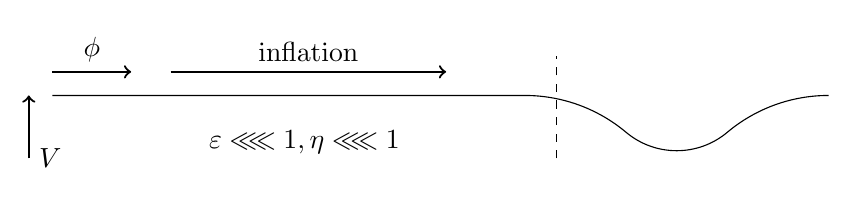
\begin{tikzpicture}
                \draw[thick,->] (-0.3,-0.8) node[right] {\(V\)} -- (-0.3,0);
                \draw[thick,->] (0,0.3) -- (1,0.3) node[midway,above] {\(\phi\)};
                \draw[thick,->] (1.5,0.3) -- (5,0.3) node[midway,above] {inflation};
                \draw (0,0) -- (6,0) arc (90:50:2) arc (230:310:1) arc (130:90:2);
                \draw[dashed] (6.4,-0.8) -- (6.4,0.5);
                \node at (3.2,-0.6) {\(\varepsilon \ll\!\!\ll 1, \eta \ll\!\!\ll 1\)};
            \end{tikzpicture}
        \end{figure}
    \item \emph{Large field} potentials have \(V''>0\) and \(V\sim \phi^n\) or \(e^{\phi/\mu}\). In this case we have \(\varepsilon \sim \frac{1}{\phi}\) or \(\frac{1}{\mu}\).
        \begin{figure}[H]
            \centering
            \begin{tikzpicture}
                \draw (0,0) .. controls (1,-6) and (3,-6) .. (4,0);
                \draw[thick,->] (3.76,0) -- (3.58,-1) node[midway,left] {\(\phi\)};
            \end{tikzpicture}
        \end{figure}
\end{itemize}
During inflation, gravitational waves are produced with an amplitude \(\sim V^{\frac14}\), so we can use this to distinguish between small and large field inflation.

The total number of e-folds of inflation we get is given by
\begin{equation}
    N_{\text{tot}} = \int_{a_i}^{a_f}\dd{\log a} = \int^{t_0}_{t_i} H \dd{t} = \int_{\phi_i}^{\phi_f} \frac1{\sqrt{2\varepsilon_V}}\frac{|\dd{\phi}|}{M_{\text{pl}}} \ge 60.
\end{equation}

Inflation ends when \(\text{KE} > \text{PE}\), and the field reaches a minimum in the potential. At this point, we can write \(V \approx \frac12m^2\phi^2\), and the Klein-Gordon equation becomes
\begin{equation}
    \ddot\phi + 3H\dot\phi + m^2\phi = 0.
\end{equation}
This has solutions of the form \(\phi = a^{-3}\cos(mt)\). Plugging these back in we find \(\expval{P_\phi} = 0\) and \(\expval{\rho_\phi} = a^{-3}\), so \(\phi\) behaves like matter.

\subsection{Issues with inflation}
We have shown that inflation solves the Horizon problem. In fact it also solves the flatness and relics problems, as these are diluted by the rapid expansion. Does inflation itself have initial condition problems? There are many very much debated features of inflation. For example, what is \(\phi\)? There are many candidates from string theory and supersymmetry. Also, is \(V\) natural; should it be so flat? And is it likely that \(\phi_i\) and \(\dot\phi_i\) allow inflation (this is the \emph{measure problem})?

Have we really solved anything? Yes: inflation has another clear prediction, and that is the production of a scale invariant spectrum of density perturbations. The field \(\phi\) has quantum fluctuations. If \(\phi\) fluctuates up the potential, its KE must decrease, so we get more inflation and a lower density, and vice versa if \(\phi\) fluctuates down the potential we get less inflation and a lower density.

We can predict the spectrum of these fluctuations. The slow-roll approximation tells us \(\dot\phi\) is approximately constant during inflation, so we spend an equal time in each \(\Delta\Phi\) interval, regardless of how much time is left in inflation. Expansion during inflation goes like \(a \sim e^{Ht}\), and each \(\Delta\Phi\) contributes an equal power to the spectrum, so we must have an equal power in each \(\log k\) interval, where \(k\) is the scale of fluctuations. Hence the spectrum is scale invariant, except for one thing: as we leave inflation, \(\dot\phi\) increases, and so there is slightly less power on small scales, resulting in a red tilt.

\section{Cosmological perturbation theory}
We want to repeat the first section, but now taking small perturbations (from e.g.\ quantum fluctuations) into account. We divide all quantities into 
\begin{equation}
    X = \underbrace{\bar{X}}_{\mathclap{\text{background}}} + \overbrace{\delta X}^{\mathclap{\text{perturbation}}}.
\end{equation}

\subsection{Perturbed metric}
We perturb the FLRW metric, and write
\begin{equation}
    \dd{s}^2 = a^2(\tau)\left[-(1+2A)\dd{\tau}^2 + 2B_i\dd{x^i}\dd{\tau} + (\delta_{ij} + h_{ij})\dd{x^i}\dd{x^j}\right],
\end{equation}
where \(A=A(\tau,x^i)\) etc.\ are small quantities. The \emph{Scalar-Vector-Tensor decomposition} is to write the small quantities as
\begin{align}
    A &\to A, \\
    B &\to \partial_iB + B^{\mathrm{V}}_i \qq{where} \partial^iB_i^{\mathrm{V}}=0, \\
    h_{ij} &\to 2C\delta_{ij} + \partial_{\langle i}\partial_{j\rangle} E + 2\partial_{(i}E^{\mathrm{V}}_{j)}+2E^{\mathrm{T}}_{ij} \\
           & \quad \qq{where} \partial^iE_i^{\mathrm{V}} = 0, \partial^iE_{ij}^{\mathrm{T}}=E^{\mathrm{T}\,i}_i=0.
\end{align}
(The \(\langle\,\rangle\) subscript notation indicates that we take the trace-free part of the object.)

Thus are perturbations are composed of:
\begin{itemize}
    \item Four scalars \(A,B,C,E\) with one degree of freedom each. These are spin 0.
    \item Two vectors \(B^{\mathrm{V}}_i\) and \(E^{\mathrm{V}}\) with two degrees of freedom each. These are spin 1, and describe rotational velocities and ``vorticity modes''.
    \item One tensor \(E^{\mathrm{T}}_{ij}\) with two degrees of freedom. These are spin 2, and describe gravitational waves.
\end{itemize}
In total, our perturbations have ten degrees of freedom.

At first order, spins don't mix, so we can treat these perturbations as being in different sectors. The vector modes are difficult to source and decay like \(a^{-2}\), so we will ignore them. We will also ignore the tensor modes/gravitational waves for now. Hence we focus on the scalars perturbations, and the metric takes the form
\begin{equation}
    \dd{s}^2 = a^2(\tau)\left(-(1+2A)\dd{\tau}^2+\partial_iB\dd{x^i}\dd{\tau} + \left[(1+2C)\delta_{ij} + 2\partial_{\langle i}\partial_{j\rangle}E\right]\dd{x^i}\dd{x^j}\right).
\end{equation}

\subsection{Gauge freedom}

In an unperturbed universe the metric is
\begin{equation}
    \dd{s}^2=a^2(\tau)(-\dd{\tau}^2+\delta_{ij}\dd{x^i}\dd{x^j}).
\end{equation}
If we change coordinates
\begin{align}
    \tilde{x}^i &= x^i + \xi^i(\tau,\vb{x}),\\
    \dd{\tilde{x}^i} &= \dd{x^i} - \partial_\tau\xi^i\dd{\tau} - \partial_k\xi^i\dd{x^k},
\end{align}
then the metric becomes
\begin{equation}
    \dd{s}^2 = a^2(\tau)\left(-\dd{\tau}^2 + 2\xi'_i \dd{\tilde{x}^i}\dd{\tau} + (\delta_{ij} + 2\partial_{(i}\xi_{j)})\dd{x^i}\dd{x^j}+O(\xi^2)\right).
\end{equation}
Similarly if we change the time coordinate to \(\tilde{\tau} = \tau + \xi^0\), then the pressure changes like
\begin{equation}
    \rho(\tilde{\tau}) = \rho(\tau+\xi^0) = \bar{\rho}(\tau) + \underbrace{\xi^0\bar{\rho}'}_{\mathclap{\text{fake density perturbation}}}.
\end{equation}
These are known as \emph{gauge modes}.

Consider now the general case \(x^\mu \to \tilde{z}^\mu+\xi^\mu(\tau,x^i)\), and write \(\xi^0 = T\), \(\xi^i=\partial_iL\). Under this transformation we have \(g_{00} = \left(\dv{\tilde{\tau}}{\tau}\right)^2\tilde{g}_{00}\), so
\begin{align}
    a^2(\tau)(1+2A) &= (1+T')^2a^2(\tau+T)(1+2\tilde{A}) \\
                    &\approx (1+2T')(a^2(\tau) + 2a'(\tau)a(\tau)T)(1+2\tilde{A}),
\end{align}
so \(A \to \tilde{A} = A-T'-\mathcal{H}T\). It is an exercise to find how the other perturbations transform. In summary, we have:
\begin{align}
    \tilde{A} &= A - T' - \mathcal{H}T \\
    \tilde{B} &= B + T - L' \\
    \tilde{C} &= C - \mathcal{H}T - \frac{1}{2}\nabla^2L \\
    \tilde{E} &= E - L
\end{align}

There are several solutions to this gauge problem:
\begin{enumerate}
    \item Just compute the observables.
    \item Follow every component through to the end and identify the gauge modes at the end.
    \item Fix the gauge. There are a few popular metric gauges:
        \begin{description}
            \item[Synchronous:] \(A=B=0\), time is unperturbed.
            \item[Spatially flat:] \(C=E=0\), space is unperturbed.
            \item[Longitudinal/Newtonian:] \(B=E=0\). This results in no diagonal part, and the spatial perturbation directly relates to the Newtonian potential.
        \end{description}
    \item Work with gauge invariant quantities, e.g\ the Bardeen potentials
        \begin{equation}
            \Psi = A + \mathcal{H}(B-E') + (B-E')' \qq{and} \Phi = -C - \mathcal{H}(B-E') + \frac13\nabla^2E.
        \end{equation}
        In the Newtonian gauge, we have \(\Psi=A\) and \(\Phi = -C\).
\end{enumerate}

\subsection{Perturbed matter}
Recall that the unperturbed energy-momentum tensor takes the form
\begin{equation}
    T\indices{^\mu_\nu} = (\rho+P)U^\mu U_\nu + P\delta^\mu_\nu.
\end{equation}
Hence when we add perturbations, we write
\begin{align}
    T\indices{^\mu_\nu} &= \bar{T}\indices{^\mu_\nu} + \delta T\indices{^\mu_\nu} \\
                        &= \bar{T}\indices{^\mu_\nu} + (\delta\rho+\delta P)\bar{U}^\mu\bar{U}_\nu + \delta P \delta^\mu_\nu + (\bar{\rho}+\bar{P})(\delta U^\mu\bar{U}_\nu + \bar{U}^\mu\delta U_\nu) + \Pi\indices{^\mu_\nu},
\end{align}
where \(\Pi\) is an arbitrary extra tensor that has been added to absorb anything that has been missed. We can absorb any parts of \(\Pi\) parallel to \(\bar{U}\) into the energy density perturbation term, and we can absorb its trace into the pressure perturbation term, so we can immediately impose
\begin{equation}
    \bar{U}^\mu\Pi\indices{^\nu_\mu} = 0 \implies \Pi\indices{^0_\mu}=0 \qq{and} \Pi\indices{^i_i}.
\end{equation}
\(\Pi\) is the anisotropic stress tensor, and since we are only considering scalar quantities, we can write \(\Pi\indices{^i_j}=\partial_{\langle i}\partial_{j\rangle}\Pi\).

Noting that \(\bar{U}^\mu=\frac1a(1,0)\), \(\bar{U}_\mu=a(-1,0)\), and using \(g_\mu\nu U^\mu U^\nu\), we can show that
\begin{equation}
    \delta g_{\mu\nu}\bar{U}^\mu\bar{U}^\nu + 2\bar{U}_\mu\partial U^\mu = -2A - 2a\delta U^0 = 0 \implies \delta U^0= -\frac1a A.
\end{equation}
Hence we write \(U^\mu = \frac1a(1-A,v^i)\), where \(v^i = \partial_i v\) (which we can write since we are only working with scalars).

Exercise: show \(U_\mu=-a(1+A,-v_i-\partial_i B)\), and additionally:
\begin{align}
    \delta T\indices{^0_0} &= -\delta\rho \\
    \delta T\indices{^0_i} &= (\bar\rho + \bar{P})\partial_i(v+B) \\
    \delta T\indices{^i_0} &= -(\bar\rho+ \bar{P})\partial^i v \equiv q^i\quad\text{(3-momentum density)} \\
    \delta T\indices{^i_j} &= \delta P \delta^i_j + \partial_{\langle i}\partial_{j\rangle}\Pi
\end{align}

In a universe with multiple components, we simply sum over the perturbations by component:
\begin{align}
    \delta\rho &= \sum_I\delta\rho_I \\
    \delta P &= \sum_I\delta P_I \\
    q^i &= \sum_I q_I \\
    \Pi &= \sum_I \Pi_I
\end{align}

Exercise: show that, under the gauge transformation defined above, the matter quantities transform as
\begin{align}
    \delta\tilde{\rho} &= \delta\rho - T\bar{\rho}', \\
    \delta\tilde{P} &= \delta P - T\bar{P}', \\
    \tilde{v} &= v + L', \\
    \tilde{\Pi} &= \Pi.
\end{align}

There are two popular matter gauges:
\begin{description}
    \item[Uniform density:] \(\delta\rho = B = 0\), spatial slices are surfaces of constant density.
    \item[Comoving:] \(v=B=0\), spatial slices move with the fluid.
\end{description}

In addition we define a gauge invariant quantity, the \emph{comoving gauge density contrast}
\begin{equation}
    \Delta = \frac{\delta\rho}{\bar{\rho}} + \frac{\bar{\rho}'}{\rho}(v+B).
\end{equation}
In comoving gauge, we have \(\Delta = \delta = \frac{\delta\rho}{\bar{\rho}}\). We call \(\delta\) the \emph{density contrast}.

\subsection{Linearised equations}
We will work in the Newtonian gauge (\(B=E=0\), \(\Psi = A\), \(\Phi = -C\)). The metric takes the simplified form
\begin{equation}
    g_{\mu\nu} = a^2(\tau)
    \begin{pmatrix}
        -(1+2\Psi) & 0 \\
        0 & (1-2\Phi)\delta_{ij}
    \end{pmatrix},
\end{equation}
and we have
\begin{equation}
    g^{\mu\nu} = \frac{1}{a^2(\tau)}
    \begin{pmatrix}
        -(1-2\Psi) & 0 \\
        0 & (1+2\Phi)\delta_{ij}
    \end{pmatrix}.
\end{equation}
Exercise: show that the components of the connection are:
\begin{align}
    \Gamma^0_{00} &= \mathcal{H}-\Psi' & \Gamma^i_{j0} &= (\mathcal{H}-\Phi')\delta^i_j \\
    \Gamma^0_{0i} &= \partial_i\Psi & \Gamma^0_{ij} &= (\mathcal{H} - \Phi' -2\mathcal{H}(\Phi+\Psi))\delta_{ij} \\
    \Gamma^i_{00} &= \delta^{ij}\partial_j\Psi & \Gamma^i_{jk} &= -2\delta^i_{(j}\partial_{k)}\Phi + \delta_{jk}\delta^{il}\partial_l\Phi
\end{align}

First we will look at the conservation equation \(\nabla_\mu T\indices{^\mu_\nu}=\partial_\mu T\indices{^\mu_\nu} + \gamma^\mu_{\mu\alpha}T\indices{^\alpha_\nu} - \Gamma^\alpha_{\mu\nu}T\indices{^\mu_\alpha}=0\). For \(\nu = 0\), to \(0^{\mathrm{th}}\) order we reobtain
\begin{equation}
    \bar{\rho}'=-3\mathcal{H}(\bar{\rho}+\bar{P}).
\end{equation}
To \(1^{\mathrm{st}}\) order, we have
\begin{equation}
    \delta\rho = \underbrace{-3\mathcal{H}(\delta\rho+\delta P)}_{\mathclap{\substack{\text{dilution due}\\\text{to expansion}}}} + \underbrace{3\Phi'(\bar{\rho}+\bar{P})}_{\substack{\text{perturbed}\\\text{expansion}}} - \underbrace{\nabla\vdot\vb{q}}_{\mathclap{\text{fluid flow}}}.
\end{equation}

Using \(\omega = \frac{P}\rho\) and \(c_s^2 = \frac{\delta P}{\delta \rho}\), we can rewrite this as
\begin{equation}
    \delta'+(1+\omega)(\nabla\vdot\vb{v}-3\Phi') + 3\mathcal{H}(c_s^2-\omega)\delta = 0.
    \tag{C}
    \label{C}
\end{equation}
This is the \emph{continuity equation}.

Now looking at \(\nu = i\), to \(1^{\mathrm{st}}\) order we have
\begin{equation}
    \vb{v}' = \underbrace{-\mathcal{H}\vb{v}}_{\mathclap{\text{redshift}}} + \underbrace{3\mathcal{H}\frac{\bar{P}'}{\bar\rho'}\vb{v}}_{\mathclap{\substack{\text{relativistic}\\\text{correction}\\\text{to redshift}}}} - \underbrace{\frac{\nabla\delta P}{\bar{\rho}+\bar{P}}}_{\mathclap{\substack{\text{pressure}\\\text{gradients}}}} - \underbrace{\nabla\Psi}_{\mathclap{\text{gravity}}}.
    \tag{E}
    \label{E}
\end{equation}
This is the \emph{Euler equation}.

Now we look at the Einstein equations. With a lot of algebra, we can deduce the components of the perturbed Einstein tensor as follows:
\begin{align}
    G_{00} &= 3\mathcal{H}^2 + 2\nabla^2\Phi - 6\mathcal{H}\Phi' \\
    G_{0i} &= 2\partial_i(\Phi' + \mathcal{H}\Psi) \\
    G_{ij} &= -(2\mathcal{H}'+\mathcal{H}^2)\delta_{ij} + \partial_i\partial_j(\Phi-\Psi) \\
           &\qquad + \left(\nabla^2(\Psi - \Phi) + 2\Phi'' + 2(2\mathcal{H}'+\mathcal{H}^2)(\Phi+\Psi) + 2\mathcal{H}\Psi' + 4\mathcal{H}\Phi'\right)\delta_{ij}
\end{align}
So now look at \(G_{\mu\nu} = 8\pi G T_{\mu\nu}\). The trace free part is
\begin{equation}
    \partial_{\langle i}\partial_{j\rangle}(\Phi-\Psi) = \partial_{\langle i}\partial_{j\rangle}\Pi.
\end{equation}
We will assume that there is no anisotropic stress, so \(\Pi=0\), and \(\Psi = \Phi\).

From the \(00\) part of the equation to \(0^{\mathrm{th}}\) order we recover the first Friedmann equation
\begin{equation}
    3\mathcal{H}^2 = 8\pi G a^2\bar\rho,
    \tag{F1}
    \label{F1}
\end{equation}
and to \(1^{\mathrm{st}}\) order we obtain
\begin{equation}
    \nabla^2\Phi = 4\pi G\bar\rho\delta + 3\mathcal{H}(\Phi'+\mathcal{H}\Phi);
    \tag{G1}
    \label{G1}
\end{equation}
this is the first \emph{gravity equation}. From the \(0i\) part or the equation to \(1^{\mathrm{st}}\) order we get the second gravity equation
\begin{equation}
    \Phi' + \mathcal{H}\Phi = -4\pi Ga^2q.
    \tag{G2}
    \label{G2}
\end{equation}
If we combine \eqref{G1} and \eqref{G2} we obtain Poisson's equation
\begin{equation}
    \nabla^2\Phi = 4\pi Ga^2\bar\rho\Delta.
    \tag{P}
    \label{P}
\end{equation}
Finally, examining the trace over the \(ij\) part to \(0^{\mathrm{th}}\) order we recover the second Friedmann equation
\begin{equation}
    2\mathcal{H}'+\mathcal{H}^2 = -8\pi G a^2\bar\rho,
    \tag{F2}
    \label{F2}
\end{equation}
and to \(1^{\mathrm{st}}\) we obtain the third gravity equation
\begin{equation}
    \Phi'' + 3\mathcal{H}\Phi' + (2\mathcal{H}'+\mathcal{H}^2)\Phi = 4\pi Ga^2\delta P.
    \tag{G3}
    \label{G3}
\end{equation}

\subsection{Adiabatic and curvature perturbations}
Since during inflation \(\dot\phi\) is approximately constant, we can view the inflaton \(\phi\) as a clock. Quantum fluctuations in \(\phi\) can then be viewed as a local time perturbation \(\delta \tau\). This is called an \emph{adiabatic} or \emph{curvature perturbation}. It induces density and pressure perturbations in all fluids taking the form
\begin{equation}
    \delta \rho_I = \bar\rho_I(\tau+\delta\tau) - \bar\rho_I = \bar\rho'_I\delta \tau.
\end{equation}
In particular we have
\begin{equation}
    \delta\tau = \frac{\delta\rho_I}{\bar\rho'_I} = \frac{\delta\rho_J}{\bar\rho'_J} = \frac{\delta P_I}{\bar{P}_I},
\end{equation}
and so
\begin{equation}
    c_s^2 = \frac{\delta P}{\delta\rho} = \frac{\bar{P}'}{\bar{\rho}'} = \dv{\bar{P}}{\bar\rho} \implies P = P(\rho).
\end{equation}
Using the background continuity equation \(\bar\rho' = -3\mathcal{H}(\bar\rho+\bar P)\), we can write
\begin{equation}
    \frac{\delta_I}{1+\omega_I} = \frac{\delta_J}{1+\omega_J}.
\end{equation}
Hence the density contrasts of all fluids are of similar size (e.g.\ \(\delta_r = \frac43\delta_m\)), and they all have the same spatial profile. Hence if we work in the constant density gauge \(\delta=0, B=0\), we set all density perturbations to zero. The perturbation is now purely in the spatial curvature; this is why they are called curvature perturbations. In this gauge it can be shown that
\begin{equation}
    a^2 R^{(3)} = -4\nabla^2\left(C-\frac13\nabla^2 E\right),
\end{equation}
where \(R^{(3)}\) is the 3D spatial Ricci scalar. Using this as a cue we tentatively define the \emph{constant density curvature perturbation} as
\begin{equation}
    \zeta = - \left[C-\frac13\nabla^2E\right]_{\delta\rho=B=0}.
\end{equation}
As it is currently defined, this quantity is not gauge invariant. Under a gauge transformation, we have
\begin{align}
    \tilde\zeta &= -\tilde{C} + \frac13\nabla^2\tilde{E}\\
                &= -C + \mathcal{H}T + \frac13\nabla^2L + \frac13\nabla^2(E-L)\\
                &= -C + \frac13\nabla^2E + \mathcal{H}T \\
                &= \zeta + \mathcal{H}T.
\end{align}
Since \(\delta\tilde{\rho} = \delta\rho-T\bar\rho'\), we can thus refine our definition of \(\zeta\) to be gauge invariant as follows:
\begin{equation}
    \zeta = -C - \frac13\nabla^2E + \mathcal{H}\frac{\delta\rho}{\bar\rho'}.
\end{equation}
In the spatially flat gauge (\(C=E=0\)), we have \(\zeta=\mathcal{H}\dd{\tau}\), and we see that this is directly related to the adiabatic perturbation.

We could equally well have used \(B\) to remove \(T\), and we would obtain the \emph{comoving curvature perturbation}
\begin{equation}
    \mathcal{R} = -C + \frac13\nabla^2E-\mathcal{H}(B+v).
\end{equation}
Both are popular. The difference between the two is proportional to the comoving gauge density contrast; we have
\begin{equation}
    \zeta-\mathcal{R} = \mathcal{H}\left(\frac{\delta\rho}{\bar\rho} + B + v\right) = \mathcal{H}\frac{\bar\rho}{\bar\rho'}\Delta = -\frac1{3(1+w)}\Delta.
\end{equation}

\eqref{P} and \eqref{F1} give
\begin{equation}
    \nabla^2\Phi = 4\pi G a^2\bar\rho\Delta = \frac{3}{2}\mathcal{H}^2\Delta,
\end{equation}
and in Fourier space this is
\begin{equation}
    \Delta_k = \frac23\left(\frac{k}{\mathcal{H}}\right)^2\Phi.
\end{equation}
On superhorizon scales (i.e.\ \(k \ll \mathcal{H}\)), we therefore have \(\Delta \to 0\), and \(\zeta \approx \mathcal{R}\).

A key property of \(\zeta\) and \(\mathcal{R}\) is that they are conserved on superhorizon scales. In the Newtonian gauge we have \(\zeta = \Phi - \frac13\frac{\delta\rho}{\bar\rho+\bar P}\). Reqrranging this and taking a time derivative, we have
\begin{equation}
    3(\bar\rho'+\bar{P}')\zeta + 3(\bar\rho + \bar P)\zeta' = 3(\bar\rho'+\bar{P}')\Phi + 3(\bar\rho+\bar P)\Phi' - \delta\rho'.
\end{equation}
Using \eqref{C}, 
\begin{align}
    3(\bar\rho'+\bar{P}')(\Phi-\zeta) &= 3\left(1+\frac{\bar{P}'}{\bar\rho'}\right)\bar\rho'(\Phi-\zeta) \\
                                      &= 3\left(1+\frac{\bar{P}'}{\bar\rho'}\right)\left[-3\mathcal{H}(\bar\rho+\bar{P})(\Phi-\zeta)\right] \\
                                      &= 3\left(1+\frac{\bar{P}'}{\bar\rho'}\right)\mathcal{H}\delta\rho,
\end{align}
and we hence have
\begin{equation}
    3(\bar\rho+\bar P)\zeta' = \underbrace{-3\mathcal{H}\left(1+\frac{\bar{P}'}{\bar\rho'}\right)\delta\rho + 3\mathcal{H}(\delta\rho+\delta P)}_{=3\mathcal{H}\left(\delta P - \frac{\bar{P}'}{\bar\rho'}\delta\rho\right) = 3\mathcal{H}\delta P_{\mathrm{nad}}} + \nabla\vdot\vb{q},
\end{equation}
were \(\delta P_{\mathrm{nad}} = \delta P - \frac{\bar{P}'}{\bar\rho'}\delta\rho\) is the non-adiabatic pressure perturbation. Thus we can write
\begin{equation}
    \zeta' = \mathcal{H}\frac{\delta P_{\mathrm{nad}}}{\bar\rho + \bar P} + \frac13\nabla\vdot\vb{v}.
\end{equation}
Note that \(\nabla\vdot\vb{v}\propto \nabla^2 v\), and \eqref{G2} tells us that \(\Phi'+\mathcal{H}^2\Phi = \frac32\mathcal{H}^2(1+w)v\), so we have
\begin{equation}
    \nabla^2v\propto \left(\frac{k}{\mathcal{H}}\right)^2(\Phi_k'+\mathcal{H}\Phi_k),
\end{equation}
which \(\sim 0\) on superhorizon scales. Hence, for adiabatic perturbations on superhorizon scales \(\zeta'=0\), i.e.\ \(\zeta\) is conserved.

\section{Structure formation}

\subsection{Perturbation evolution}
\subsubsection*{Initial conditions}
We assume that perturbations are adiabatic. Taking \eqref{G3}\(+w\)\eqref{G1}, and using \(w\)\eqref{F1}\(+\)\eqref{F2} to remove terms, we obtain (in Fourier space)
\begin{equation}
    \Phi_k'' + 3(1+w)\mathcal{H}\Phi'_k + wk^2\Phi_k=0.
\end{equation}
On superhorizon scales, we can neglect the \(k^2\) part, and the non-decaying solution is just \(\Phi=\text{constant}\). We can neglect derivatives in \eqref{G1} to get \(-3\mathcal{H}^2\Phi=\frac32\mathcal{H}^2\delta\), so \(\delta = -2\Phi\) is constant. 

Using \eqref{P} we have \(\nabla^2\Phi = \frac32\mathcal{H}^2\Delta\), so in Fourier space we have \(\Delta_k= \frac23\left(\frac{k}{\mathcal{H}}\right)^2\Phi \propto (k\tau)^2 \Phi \approx 0\) on superhorizon scales.

On subhorizon scales, we have
\begin{equation}
    \Delta = \delta - 3(1+w)\underbrace{\left(\frac{\mathcal{H}}{k}\right)}_{\text{small}} \approx \delta.
\end{equation}

On superhorizon scales, we have
\begin{equation}
    \zeta = \Phi - \frac{1}{3(1+w)}\delta = \frac{5+3w}{3+3w}\Phi,
\end{equation}
so \(\zeta = \frac32\Phi_{\text{RD}} = \frac53\Phi_{\text{MD}}\). Notably, we have \(\Phi_{\text{MD}}=\frac9{10}\Phi_{\text{RD}}\).

\subsubsection*{Evolution of \texorpdfstring{$\Phi$}{Phi}}
We are interested only in non-decaying modes. 

During radiation domination (\(w=\frac{1}{3}\)), we have
\begin{equation}
    \Phi''_k + \frac{4}{\tau}\Phi_k' + \frac{k^2}{3}\Phi_k = 0.
\end{equation}
The non-decaying solution to this equation is of the form
\begin{equation}
    \Phi_k(\tau) = 2\zeta(0)\left(\frac{\sin x-x\cos x}{x^3}\right) \qq{where} x = \frac{k\tau}{\sqrt{3}}.
\end{equation}
On superhorizon scales, we can take \(x\) to be small and \(\Phi_k(\tau)\approx \frac23\zeta(0)\). On subhorizon scales we have \(\Phi_k(\tau) = 6\zeta(0)\frac{\cos x}{x^2} \sim \frac{\text{oscillations}}{a^2}\) (during radiation domination \(a \sim \tau\)).

During matter domination (\(w=0\)), the equation is
\begin{equation}
    \Phi''_k + \frac{6}{\tau}\Phi'_k=0,
\end{equation}
and the only ungrowing mode is \(\Phi_k=\text{constant}\), for both subhorizon and superhorizon scales.

To summarise:
\begin{figure}[H]
    \centering
    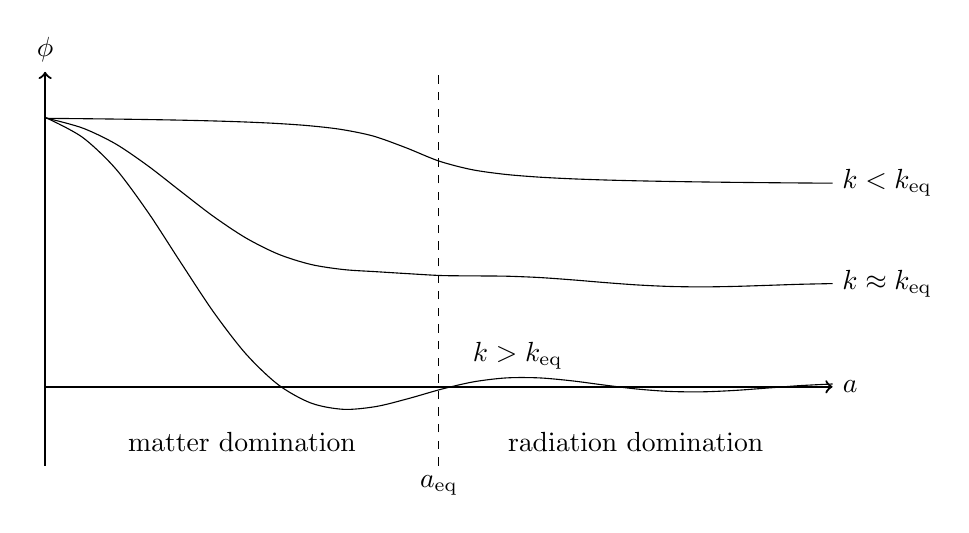
\begin{tikzpicture}
        \draw[thick,->] (0,0) -- (10,0) node[right] {\(a\)};
        \draw[thick,->] (0,-1) -- (0,4) node[above] {\(\phi\)};
        \draw[domain=0.1:15,smooth,variable=\x] (0,3.42) -- plot({\x/1.5},{10*(sin(360*\x/(2*pi))-\x*cos(360*\x/(2*pi)))/(\x^3)});
        \node[above] at (6,0.1) {\(k>k_{\mathrm{eq}}\)};
        \draw[domain=0:15,smooth,variable=\x] plot({\x/1.5},{3-atan(\x - 7)/200}) node[right] {\(k < k_{\mathrm{eq}}\)};
        \draw[domain=0.1:15,smooth,variable=\x] (0,3.42) -- plot({\x/1.5},{0.5*(3-atan(\x - 7)/200+ 10*(sin(360*\x/(2*pi))-\x*cos(360*\x/(2*pi)))/(\x^3))}) node[right] {\(k \approx k_{\mathrm{eq}}\)};
        \draw[dashed] (5,-1) node[below] {\(a_{\mathrm{eq}}\)} -- (5,4);
        \node at (2.5,-0.7) {matter domination};
        \node at (7.5,-0.7) {radiation domination};
    \end{tikzpicture}
\end{figure}

\subsubsection*{Evolution of radiation}
During radiation domination, \eqref{P} tells us that
\begin{equation}
    \nabla^2\Phi = \frac32\mathcal{H}\Delta_r \implies \Delta_r = -\frac23\left(\frac{k}{\mathcal{H}}\right)^2\Phi_k \propto a^2\Phi_k.
\end{equation}
Hence on superhorizon scales \(\Delta_r \propto a^2\) and on subhorizon scales \(\Delta_r(\approx\delta_r) = -4\zeta(0)\cos\frac{k\tau}{\sqrt{3}}\).

During matter domination, radiation is subdominant, so we need to use \eqref{C} and \eqref{E} to find its evolution. \(\Phi\) is constant in time, so we have
\begin{equation}
    \delta_r'=-\frac43\nabla\vdot\vb{v}_r \qq{and} \vb{v}_r'=-\frac14\nabla\delta_r - \nabla\Phi.
\end{equation}
Combining these two, we obtain
\begin{equation}
    \delta_r'' - \frac13\nabla^2\delta_r = \frac43\nabla^2\Phi.
\end{equation}
The RHS is constant in time, so this is just a forced wave equation. The solution is \(\delta_r = -4\Phi + \text{oscillations}\).

\subsubsection*{Evolution of dark matter}
During matter domination, we can use \eqref{P}:
\begin{equation}
    \nabla^2\Phi=\frac32\mathcal{H}\Delta_m\implies\Delta_m = -\frac23\left(\frac{k}{\mathcal{H}}\right)^2\Phi \sim \tau^2 \sim a
\end{equation}
This holds on all scales.

When radiation is also present, we must make use of \eqref{C} and \eqref{E}:
\begin{equation}
    \delta_m'=-\nabla\vdot\vb{v}_m + 3\Phi',\quad\vb{v}_m' = \mathcal{H}\vb{v}_m - \nabla\Phi
\end{equation}
We split the potential into its raidation and matter parts, \(\Phi = \Phi_r + \Phi_m\). On subhorizon scales, we know that \(\Phi_r\sim\cos(k\tau)\sim\cos(k/\mathcal{H})\) (and \(k/\mathcal{H}\) is large so we get fast oscillations) and \(\Phi_m\sim\text{constant}\). The ``fast'' (radiation) mode of \(\delta_m\) is suppressed by a factor of \(\left(\frac{\mathcal{H}}{k}\right)^2\) relative to the ``slow'' (matter) mode. Thus we can take \(\Phi \approx \Phi_m\), neglecting \(\Phi_r\), and write
\begin{equation}
    \Phi'\approx\Phi''\approx0,\quad\nabla^2\Phi\approx\frac32\mathcal{H}^2\Delta_m\approx\frac32\mathcal{H}^2\delta_m.
\end{equation}
Combining these with the above, we obtain 
\begin{equation}
    \delta_m''+ \mathcal{H}\delta_m' - \frac32\mathcal{H}^2\delta_m=0.
\end{equation}
In a universe with only radiation and matter, we have
\begin{equation}
    \mathcal{H}^2 = \frac{\mathcal{H}_0^2\Omega_m^2}{\Omega_r}\left(\frac1y+\frac1{y^2}\right),
\end{equation}
where \(y = \frac{a}{a_{\text{eq}}}\). Substituting this into the above, we obtain the \emph{M\'esz\'aros equation}:
\begin{equation}
    \dv[2]{\delta_m}{y} + \frac{2+3y}{2y(1+y)}\dv{\delta_m}{y} - \frac3{2y(1+y)}\delta_m = 0.
\end{equation}
The solutions are of the form
\begin{equation}
    \delta_m \propto
    \begin{cases}
        2+3y, \\
        (2+3y)\log\left(\frac{\sqrt{1+y}+1}{\sqrt{1+y}-1}\right) - 6\sqrt{1+y}.
    \end{cases}
\end{equation}
Hence we see for radiation domination (\(y\ll1\)), \(\delta_m\propto\log y\propto\log a\) (growth stalls), and for matter domination (\(y\gg1\)), \(\delta_m\propto y\propto a \propto \tau^2\).

\subsubsection*{Evolution of baryons}
During radiation domination, baryons are tightly coupled to photons by Thompson scattering. Hence we can write \(\Delta_b \sim \Delta_\gamma \propto \Delta_r\), so \(\Delta_b\) oscillates with \(\Delta_r\).

During matter domination, baryons have pressure, so \eqref{C} and \eqref{E} on subhorizon scales provides
\begin{equation}
    \delta_b'' + \mathcal{H}\delta_b' - c_s^2\nabla^2\delta_b = \nabla^2\Phi.
\end{equation}
This is the same as the equation for dark matter with \(c_s=0\), so if we define \(\delta_b-\delta_c = \delta_{bc}\), then we can write this as (in Fourier space)
\begin{equation}
    \delta''_{bc} + \mathcal{H}\delta'_{bc} = -c_s^2k^2\delta_b.
\end{equation}
If \(k\ll\frac{1}{c_s}\) (i.e.\ for modes larger than the sound horizon), we have \(\delta_{bc}\) constant. Since \(\delta_m \propto a\), \(\frac{\delta_{bc}}{\delta_m}\propto\frac1a\), so the difference is negligible. Thus on scales larger than the sound horizon, baryons follow matter. 

For scales smaller than the sound horizon, we can write
\begin{equation}
    \delta_b'' + \mathcal{H}\delta_b + c_s^2k^2\delta_b = \nabla^2\Phi = \frac32\mathcal{H}^2\delta_m \approx \frac32\mathcal{H}^2\delta_b,
\end{equation}
so
\begin{equation}
    \delta_b'' + \mathcal{H}\delta_b' + \left(c_s^2 k^2 - \frac32\mathcal{H}^2\right)\delta_b = 0.
\end{equation}
This defines a critical wavenumber \(k=\sqrt{\frac32}\frac{\mathcal{H}}{c_s}\), or alternatively a critical wavelength \(\lambda_J = a\lambda = c_s\sqrt{\frac{\pi}{G\bar{\rho}}}\); this is the \emph{Jeans length}. For \(\lambda>\lambda_J\), structure collapses. For \(\lambda < \lambda_J\), structure is supported by baryonic pressure.

At some point baryons switch from being supported by the radiation to being supported by matter. We call this event \emph{recombination}; it is when atoms combine and baryons decouple from photons. We will indicate it with a \(*\). At late times in matter domination we have
\begin{equation}
    \Delta_c \approx \Delta_b \approx \Delta_m = \Delta^*_m\left(\frac{a}{a^*}\right) = \left(f_b\Delta_b^* + f_c\Delta_c^*\right)\left(\frac{a}{a^*}\right),
\end{equation}
where \(f_X = \frac{\bar{\rho}_X}{\bar{\rho}}\) is the \emph{fractional density} of \(X\). Thus we have
\begin{equation}
    \Delta_m \approx \frac{1}{f_c}\Delta_c\left(1+\epsilon\cos\left(\frac{k\tau^*}{\sqrt{3}}\right)\right),
\end{equation}
for some small constant \(\epsilon\). These small oscillations are called \emph{Baryon Accoustic Oscillations} (BAO) and measuring them provides a value of \(\tau^*\), the time of recombination.

\subsubsection*{Summary of perturbation evolutions}
This table summarises subhorizon perturbation evolutions:
\begin{table}[H]
    \centering
    \begin{tabular}{lcc}
        \toprule
        & Radiation domination & Matter domination \\
        \midrule
        Potential \(\Phi\) & \(a^{-2}\cos(\frac{k\tau}{\sqrt3})\) & constant \\
        Radiation \(\delta_r\) & \(\cos(\frac{k\tau}{\sqrt3})\) & \(A\cos(\frac{k\tau}{\sqrt3})-4\Phi_{\text{MD}}\) \\
        Matter \(\delta_m\) & \(\log \tau\) & \(\tau^2\) \\
        Baryons \(\delta_b\) & \(\cos(\frac{k\tau}{\sqrt3})\) & \(\tau^2\) \\
        \bottomrule
    \end{tabular}
\end{table}
\(\Phi\) and \(\delta\) are constant on superhorizon scales for both radiation and matter domination. Also:
\begin{equation}
    \Delta = 
    \begin{cases}
        \delta \tau^2 & \text{superhorizon} \\
        \delta & \text{subhorizon}
    \end{cases}
\end{equation}

\subsection{Power spectra}
We know the evolution of all fluid perturbations in all eras. How do we measure them? We assume that the perturbations are Gaussian (as the primal fluctuations are Gaussian and we are in a linear regime), so they are completely described by their \emph{power spectra} \(P\), defined by
\begin{equation}
    \expval{X(\vb{k})X^*(\vb{k}')} = (2\pi)^3\delta(\vb{k}-\vb{k}')P_X(k).
\end{equation}
The power spectrum simply gives the variance at a particular scale \(k\).

\subsubsection*{Initial conditions}
Recall that curvature perturbations from initial conditions have equal power in log intervals, i.e.\ \(P_\zeta(\tau_i,k)\) is scale invariant. In other words, the power in the interval \([k_1,k_2]\) is proportional to \(\log k_2 - \log k_1\). Since
\begin{equation}
    \int^{k_2}_{k_1}P(k)\dd[3]{k} = 4\pi\int^{k_2}_{k_1} P(k) k^2\dd{k} =  4\pi\int^{\log k_2}_{\log k_1} k^3P(k)\dd{(\log k)},
\end{equation}
we must have that \(P_\zeta(k)\propto k^{-3}\). The claim of scale invariance is not exactly true, so we define \(P_\zeta(k) = A_\zeta k^{n_s-4}\), where \(n_s\) is the \emph{spectral tilt}. For \(n_s=1\) we recover scale invariance.

\subsubsection*{Matter}
If we plot the previous results for matter perturbation evolution on the \(k\)-\(\tau\) plane, we observe two distinct regions:

\begin{figure}[H]
    \centering
    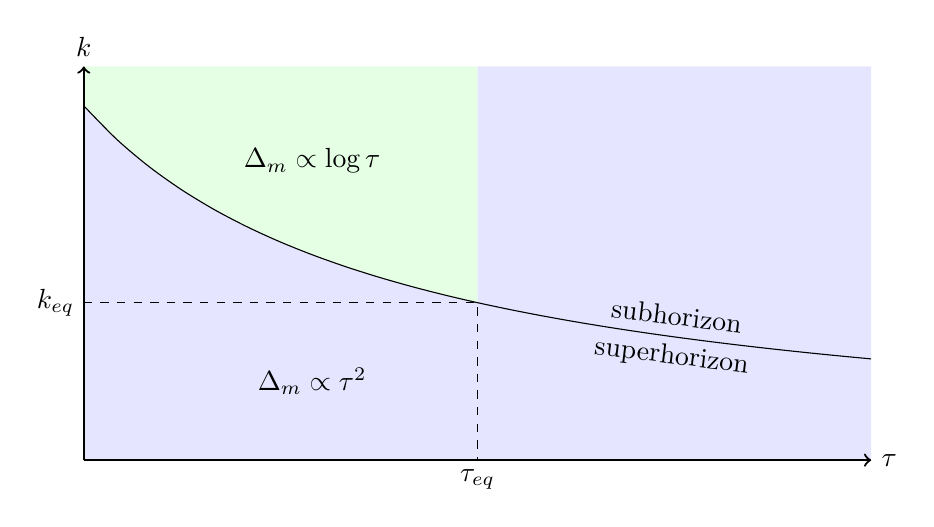
\begin{tikzpicture}
        \fill[green!10,domain=5:0,smooth,variable=\x] (5,5) -- (5,2) plot({\x},{18/(\x+4)}) -- (0,5) -- (5,5);
        \fill[blue!10,domain=5:0,smooth,variable=\x] (0,0) -- (10,0) -- (10,5) -- (5,5) -- (5,2) plot({\x},{18/(\x+4)}) -- (0,0);
        \node at (2.9,3.8) {\(\Delta_m\propto \log\tau\)};
        \node at (2.9,1) {\(\Delta_m\propto \tau^2\)};
        \draw[thick,->] (0,0) -- (10,0) node[right] {\(\tau\)};
        \draw[thick,->] (0,0) -- (0,5) node[above] {\(k\)};
        \draw[domain=0:10,smooth,variable=\x] plot({\x},{18/(\x+4)});
        \node[above, rotate={-7}] at (7.5,1.59) {subhorizon};
        \node[below, rotate={-7}] at (7.5,1.59) {superhorizon};
        \draw[dashed] (0,2) node[left] {\(k_{\text{eq}}\)} -- (5,2) -- (5,0) node[below] {\(\tau_{\text{eq}}\)};
    \end{tikzpicture}
\end{figure}

Note that at initial times everything is superhorizon and we have \(\Delta_m \propto \left(\frac{k}{\mathcal{H}}\right)^2\Phi\propto\left(\frac{k}{\mathcal{H}}\right)^2\zeta\), so we can write \(P_{\Delta_m}(\tau_i,k)\propto k^4P_\zeta(\tau_i,.k)\).

Modes with \(k<k_{\text{eq}}\) are always in the region with \(\Delta_m \propto \tau^2\). Hence we can immediately write
\begin{equation}
    P_{\Delta_m}(\tau_0,k<k_{\text{eq}}) = \left(\frac{\tau_0}{\tau_i}\right)^4P_{\Delta_m}(\tau_i,k) \propto k^4P_\zeta \propto k^{n_s}.
\end{equation}

Modes with \(k>k_{\text{eq}}\) must travel through the \(\Delta_m \propto \log \tau\), so if we define \(\tau_{\text{HX}} \sim \frac1k\) as the time at which the mode crosses the horizon, we have
\begin{equation}
    P_{\Delta_m}(\tau_0,k>k_{\text{eq}}) = \left(\frac{\tau_0}{\tau_{\text{eq}}}\right)^4 \left(\frac{\log \tau_{\text{eq}}}{\log\tau_{\text{HX}}}\right)^2\left(\frac{\tau_{\text{HX}}}{\tau_i}\right)^4P_{\Delta_m}(\tau_i,k) \propto k^{n_s-4}\log^2k .
\end{equation}
We should also include a factor of \(\left(1+2\epsilon\cos(\frac{k\tau^*}{\sqrt3})\right)^2\) that comes from BAO. 

\subsubsection*{Radiation}
This treatment is crude AF as we are neglecting baryons. As before we have \(P_{\Delta_r}(\tau_i,k)\propto k^4P_\zeta(\tau_i,k) \propto k^{n_s}\). Now we have three regions:
\begin{figure}[H]
    \centering
    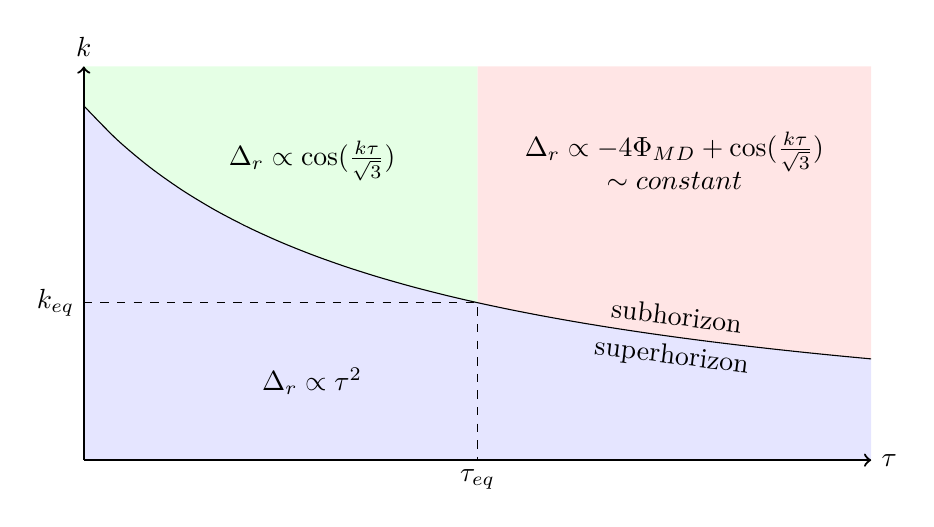
\begin{tikzpicture}
        \fill[green!10,domain=5:0,smooth,variable=\x] (5,5) -- (5,2) plot({\x},{18/(\x+4)}) -- (0,5) -- (5,5);
        \fill[red!10,domain=5:10,smooth,variable=\x] (5,5) -- (5,2) plot({\x},{18/(\x+4)}) -- (10,5) -- (5,5);
        \fill[blue!10,domain=10:0,smooth,variable=\x] (0,0) -- (10,0) -- (10,{18/14}) plot({\x},{18/(\x+4)}) -- (0,0);
        \node at (2.9,3.8) {\(\Delta_r\propto \cos(\frac{k\tau}{\sqrt3})\)};
        \node[align=center] at (7.5,3.8) {\(\Delta_r\propto -4\Phi_{\text{MD}} + \cos(\frac{k\tau}{\sqrt3})\)\\\(\sim \text{constant}\)};
        \node at (2.9,1) {\(\Delta_r\propto \tau^2\)};
        \draw[thick,->] (0,0) -- (10,0) node[right] {\(\tau\)};
        \draw[thick,->] (0,0) -- (0,5) node[above] {\(k\)};
        \draw[domain=0:10,smooth,variable=\x] plot({\x},{18/(\x+4)});
        \node[above, rotate={-7}] at (7.5,1.59) {subhorizon};
        \node[below, rotate={-7}] at (7.5,1.59) {superhorizon};
        \draw[dashed] (0,2) node[left] {\(k_{\text{eq}}\)} -- (5,2) -- (5,0) node[below] {\(\tau_{\text{eq}}\)};
    \end{tikzpicture}
\end{figure}
Repeating the kind of analysis used before, we have
\begin{equation}
    P_{\Delta_r}(\tau_0,k<k_{\text{eq}}) = \left(\frac{\tau_{\text{HX}}}{\tau_i}\right)^4P_{\Delta_r}(\tau_i,k) \propto \frac{1}{k^4} k^4 P_\zeta \propto k^{n_s-4},
\end{equation}
and
\begin{equation}
    P_{\Delta_r}(\tau_0,k>k_{\text{eq}}) = \left(\frac{\tau_{\text{HX}}}{\tau_i}\right)^4 \cos^2(\frac{k\tau_{\text{eq}}}{\sqrt3}) P_{\Delta_r}(\tau_i,k) \sim \frac{1}{k^4}\cos^2(k) k^4 P_\zeta \sim k^{n_s-4} \cos^2 k.
\end{equation}

\subsection{Spherical collapse}
To determine how collapsed objects form we need to go beyond linear theory. Consider flat FLRW with only matter. Take a spherical region of radius \(\bar{R}\) and compress it a small amount to a spherical region of radius \(R\).

\begin{figure}[H]
    \centering
    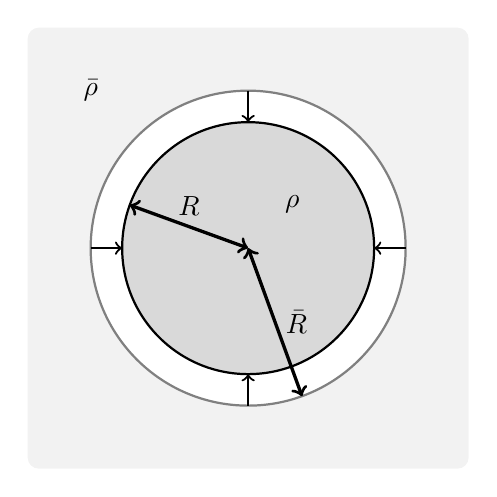
\begin{tikzpicture}[scale=0.8]
        \fill[gray!10,rounded corners] (-3.5,-3.5) rectangle (3.5,3.5);
        \draw[gray,thick,fill=white] (0,0) circle (2.5);
        \draw[thick,fill=gray!30] (0,0) circle (2);
        \draw[thick,->] (2.5,0) -- (2,0);
        \draw[thick,->] (-2.5,0) -- (-2,0);
        \draw[thick,->] (0,2.5) -- (0,2);
        \draw[thick,->] (0,-2.5) -- (0,-2);
        \draw[very thick, <->, rotate=-70] (0,0) -- (2.5,0) node[midway,right] {\(\bar{R}\)};
        \draw[very thick, <->, rotate=160] (0,0) -- (2,0) node[midway,above] {\(R\)};
        \node at (0.7,0.7) {\(\rho\)};
        \node at (-2.5,2.5) {\(\bar{\rho}\)};
    \end{tikzpicture}
\end{figure}
The spherical mass theorem implies that the background is unperturbed, so \(\bar{R}\propto a\propto t^{\frac23}\) and \(\bar{\rho}\propto\frac1{t^2}\). It also implies that the compressed sphere is independent of the background, so it evolves like an FLRW closed universe with \(\rho>\rho_{\text{crit}} = \bar\rho\). The radius of the sphere evolves via \eqref{F1}:
\begin{equation}
    \dot{R} = \frac{\Omega_{m,0}}{R^2} - k
\end{equation}
This has the solution
\begin{equation}
    R = A(1-\cos\theta) \qq{and} t=B(\theta-\sin\theta),
\end{equation}
where \(A = \frac{\Omega_{m,0}}{2\Omega_{m,0}-1}\), \(B = \frac{\Omega_{m,0}}{2H_0(\Omega_{m,0}-1)^{\frac32}}\) and \(\theta \in [0,2\pi)\). Expanding to leading order in \(\theta\), we have \(R\approx A\frac{\theta^2}{2}\) and \(t\approx B\frac{\theta^3}{6}\), so \(R\propto t^{\frac23}\), just like the background. Expanding to the next order, we have
\begin{equation}
    R\approx A \frac{\theta^2}{2}\left(1-\frac{\theta^2}{12}\right) \qq{and} t \approx B\frac{\theta^3}{6}\left(1-\frac{\theta^2}{20}\right),
\end{equation}
so we can write
\begin{equation}
    R\approx \frac{A}{2}\left(\frac{6t}{B}\right)^{\frac23}\left(1-\frac1{20}\left(\frac{6t}{B}\right)^{\frac23}\right) = \bar{R}(1+\delta_R)
\end{equation}
where \(\delta_R  = -\frac1{20}\left(\frac{6t}{B}\right)^{\frac23}\). Using mass conservation we have
\begin{equation}
    \rho_IR_I^3 = \rho R^3 \approx \rho_I(1+\delta)\bar{R}^3(1+3\delta_R) \implies \delta \approx -3\delta_R \propto a,
\end{equation}
as we see in the linear theory. 

There are a couple of key points in the evolution of the perturbation. The linear theory predicts values of \(\delta\) for these points:
\begin{itemize}
    \item \emph{Turnaround} at \(\theta=\pi\), \(t=\pi B\), \(\delta\approx1.06\).
    \item \emph{Collapse} at \(\theta=2\pi\), \(t=2\pi B\), \(\delta\approx1.69\).
\end{itemize}
These are clearly incorrect as linear approximations have become inaccurate. However, the values can be useful. When a linear perturbation grows beyond \(\delta > 1.69\) we expect to see a collapsed object. What do the collapsed objects look like? At turnaround (\(\theta=\pi\)), we have
\begin{equation}
    1+\delta_{\text{turn}} = \frac{\rho}{\bar\rho} = \frac{\Omega_{m,0}\bar\rho_0\frac{1}{R^3}}{\bar\rho_0\frac{1}{a^3}} = \Omega_{m,0} \left(\frac{a}{R}\right)^3.
\end{equation}
Using \(a=\left(\frac32 H_0 t\right)^{\frac23}\), \(R=2A\) and \(t=\pi B\), we hence have
\begin{equation}
    1+\delta_{\text{turn}} = \frac{9\pi^2}{16} = 5.55.
\end{equation}

Formally at \(\theta = 2\pi\), \(\rho\to \infty\) and so \(\delta \to \infty\). In reality, collapse stops due to ``virialisation'': dissipative processes convert kinetic energy to random motion. The system stabilises when random motion balances the potential, and the virial theorem states that this stability is reached when \(V=-2K\), where \(V\) is the potential energy and \(K\) is the kinetic energy.

At turnaround, things are stationary so the total energy is \(E=V\) and \(K=0\). At virialisation, \(E=V=K=-K\implies V=2E\), so collapse stops when the potential energy has doubled. \(V\to 2V\) corresponds to \(R\to \frac12 R\) and \(\rho \to 8\rho\). From turnaround, \(\bar\rho\) has decreased by \(\left(\frac{a_{\text{turn}}}{a_{\text{vir}}}\right)^3 = \left(\frac{t_{\text{turn}}}{t_{\text{vir}}}\right)^2 = 4\), and hence we have
\begin{equation}
    \frac{\rho_{\text{vir}}}{\bar\rho} = 1 + \delta_{\text{vir}} \approx 5.55\times8\times4 \approx 178.
\end{equation}

In summary, in linear theory perturbations grow until \(\delta > 1.69\), at which point we can replace them with virialised \emph{halos} with \(\rho \sim 200 \bar\rho\).

\subsection{Filtering}
To apply the results of the previous section we need to smooth \(\delta\) on the lengthscale \(R\). To do this we make things convoluted with a window function \(W\), writing
\begin{equation}
    \delta_R(t,\vb{x}) = \int \delta(t,\vb{x}') W(|\vb{x}-\vb{x}'|,R) \dd[3]{x'},
\end{equation}
or in Fourier space
\begin{equation}
    \delta_R(t,\vb{k}) = \delta(t,\vb{k}) \tilde{W}(R,\vb{k}).
\end{equation}
The choice of window function is fairly arbitrary, but here are some popular ones:
\begin{itemize}
    \item \emph{Top hat}:
        \begin{equation}
            W_{\text{TH}} = 
            \begin{cases}
                \frac{3}{4\pi R^3} & r \le R \\
                0 & r > R
            \end{cases},
            \quad
            \tilde{W}_{\text{TH}} = \frac3{(kR)^3}\left[\sin(kR) - kR \cos(kR)\right]
        \end{equation}
    \item \emph{Gaussian}:
        \begin{equation}
            W_{\text{G}} = \frac1{(2\pi)^{\frac32} R^3}\exp(\frac{-r^2}{2R^2}),\quad
            \tilde{W}_{\text{G}} = \exp(-\frac{(kR)^2}2)
        \end{equation}
    \item \emph{\(k\)-space cut}:
        \begin{equation}
            W_k = \frac1{2\pi^2r^3}\left(\sin(\frac{r}{R}) - \frac{r}{R} \cos(\frac{r}{R})\right),\quad
            \tilde{W}_k = 
            \begin{cases}
                1 & k < \frac1R \\
                0 & k > \frac1R
            \end{cases}
        \end{equation}
\end{itemize}

We assume that \(\delta\) is Gaussian (as we are in a linear regime), so we can describe its statistics in two quantities, its mean and its variance. The mean \(\bar{\delta}=\expval{\delta}\) is by definition equal to zero, so we have \(\bar\delta_R = 0\). Also we have
\begin{equation}
    \sigma_R^2 = \expval{\delta_R\delta_R} = \frac1{2\pi^2}\int P(k)\tilde{W}^2(kR)k^2\dd{k}.
\end{equation}
From this we define the following important cosmological parameter:
\begin{equation}
    \sigma_8 = \sqrt{\frac1{2\pi^2} \int P_{\text{lin}}(k)\tilde{W}_{\text{TH}}^2(kR) k^2\dd{k}} \qq{where} R=8h^{-1}\si{\mega\parsec}
\end{equation}
\(\sigma_8^2\) is the variance of the linear density field on \(8h^{-1}\si{\mega\parsec}\) scales. We observe \(\sigma_8\approx0.8\). If \(\sigma_8\) were larger, we would have larger fluctuations and earlier structure formation, and vice versa. Recall that
\begin{equation}
    P_{\text{lin}}(k) \propto
    \begin{cases}
        k^{n_s} & k < k_{\text{eq}}, \\
        k^{n_s-4}\log^2k & k > k_{\text{eq}}.
    \end{cases}
\end{equation}
We define the \emph{effective spectral index} \(n_{\text{eff}}\) by \(P_{\text{lin}}(l) = A^2(t)k^{n_{\text{eff}}(k)}\), where \(A(t) \propto a(t)\). If we set \(y=kR\) and assume that \(n_{\text{eff}}\) is constant on relevant scales, we have
\begin{equation}
    \sigma_R^2 = \frac{A^2(t)}{2\pi^2} \int k^{n_{\text{eff}}+2} \tilde{W}^2(kR)\dd{k} = \frac{A^2(t)}{2\pi^2} \frac{1}{R^{n_{\text{eff}}+e}} \int y^{n_\text{eff}+2} \tilde{W}^2(y)\dd{y},
\end{equation}
wheer \(n_{\text{eff}}\) is evaluated at \(k=\frac{2\pi}{R}\). In the range of interest \(0.8\si{\mega\parsec}\to40\si{\mega\parsec}\), the integral over \(y\) is approximately constant, so we have \(\sigma_R \propto A(t) R^{-(n_{\text{eff}}+3)/2}\). Converting this to mass \(M(R) \propto R^3\), we have \(\sigma_M \propto A(t) M^{-(n_{\text{eff}}+3)/6}\).

\subsection{Press-Schechter mass function}
We want to calculate the number density of halos for a given mass range. We assume that the probability that \(\delta_M(t)>\delta_c = 1.69\) is equivalent to the mass fraction at time \(t\) contained in halos with mass \(>M\). Since \(\delta_M\) is Gaussian, we have
\begin{equation}
    P(\delta_M>\delta_c) = \frac1{\sqrt{2\pi}\sigma_M} \int^\infty_{\delta_c}\exp(\frac{-x^2}{2\sigma^2_M})\dd{x} = \frac12 \operatorname{erfc}\left(\frac{\delta_c}{\sqrt2 \sigma_M}\right) = \frac12\operatorname{erfc}\left(\frac\nu{\sqrt{2}}\right),
\end{equation}
where \(\nu = \frac{\delta_c}{\sigma_M}\). But there's something stupidly wrong here; if we take the limit as \(M\) goes down to \(0\), then \(\sigma \to \infty\) and \(P \to \frac12\), which is not true -- it should be \(1\). So be inspired and pretend that \(P=2P\), so that we instead take \(P=\operatorname{erfc}\left(\frac\nu{\sqrt2}\right)\). 

Let \(\bar{n}_h(M)\) denote the mean number of halos of mass \(M\) per unit of comoving volume. The volume taken by a halo of mass \(M\) is \(V_M = \frac{M}{\bar\rho}\). Also the fraction of halos with mass in the range \([M,M+\Delta M]\) is \(-\dv{P}{M}\Delta M\). Hence we have
\begin{equation}
    \dv{\bar{n}_h}{M} = -\frac1{V_M}\dv{P}{M} = - \frac{\bar\rho}{M}\dv{P}{\sigma_M}\dv{\sigma_M}{M}.
\end{equation}
Putting in the above value for \(P\) we have the \emph{Press-Schechter mass function}:
\begin{equation}
    \dv{\bar{n}_h}{M} = -\sqrt{\frac{2}{\pi}} \frac{\bar\rho}{M\sigma_M} \dv{\sigma_M}{M} \nu e^{-\frac{\nu^2}{2}}
\end{equation}
Writing \(\frac{\nu}{\sqrt{2}} = \frac{\delta_c}{\sqrt{2}\sigma_M} \propto B(t) M^{(3+n_{\text{eff}})/6}\) and \(\gamma = 1 + \frac{n_{\text{eff}}}{3}\), we can find
\begin{equation}
    \dv{\bar{n}_h}{M} \approx \gamma \frac{B(t)}{\sqrt{\pi}}\frac{\bar\rho}{M^2} M^{\gamma/2} \exp(-B^2(t) M^\gamma).
\end{equation}
For small \(M\) we get a power law, and for large \(M\) we get an exponential cutoff.

\subsection{Linear bias}
How do the statistics of halos relate to the statistics of the linear perturbation? We define the Halo overdensity by
\begin{equation}
    \delta_h = \frac{n_h-\bar{n}_h}{\bar{n}_h}.
\end{equation}
The corresponding halo-halo correlation is 
\begin{equation}
    \xi_{hh}(r=|\vb{x}-\vb{x}'|) = \expval{\delta_h(\vb{x}),\delta_h(\vb{x}')} = \frac{\expval{n_h(\vb{x}),n_h(\vb{x}')}}{\bar{n}_h^2} - 1.
\end{equation}
We make a peak-background split \(\delta=\delta_h+\delta_b\). \(\delta_h\) contains short wavelength halos, and \(\delta_b\) contains long wavelength background perturbations.

Locally, collapse occurs when \(\delta_h > \tilde{\delta}_c = \delta_c = \delta_b\), and happens around an approximately constant background density \(\tilde\rho = \bar\rho(1+\delta_b)\). \(\tilde{\delta}_c\) and \(\tilde{\rho}\) are both functions of \(\delta_b\). Expanding \(\dv{\bar{n}_h}{M}\) about \(\delta_b\), we have
\begin{align}
    \dv{\bar{n}_h}{M} &= \dv{\bar{n}_h}{M} + \left(\pdv{\tilde{\delta}_c}\dv{\bar{n}_h}{M}\dv{\tilde\delta_c}{\delta_b} + \pdv{\tilde\rho}\dv{\bar{n}_h}{M}\dv{\tilde\rho}{\delta_b}\right)\delta_b + \dots \\
                      &= \dv{\bar{n}_h}{M} \left( 1 + \left(1+\frac{\nu^2-1}{\nu\sigma_M}\right)\delta_b\right) + \dots \\
                      &\approx b(M) \dv{\bar{n}_h}{M},
\end{align}
where we have defined \(b(M) = 1 + \frac{\nu^2-1}{\delta_c}\), the \emph{linear bias}. Now we can relate the two point halo correlator to the correlator for the linear field by
\begin{equation}
    \xi_{hh}(r,M) = b^2(M) \xi_{\text{linear}}(r).
\end{equation}

\section{Big Bang Cosmology}
\subsection{The hot big bang}
Local equilibrium in an expanding universe requires \(\Gamma \gg H\), where \(\Gamma = n \sigma v\) is the interaction rate of the species in equilibrium, and \(n\) is the number of density of target particles, \(\sigma\) the cross section of interactions and \(v\) the relative velocity. For example:
\begin{itemize}
    \item For \(T \gg 100\si{\giga\eV}\), all particles are relativistic with \(v \sim 1\). By dimensional anaylsis, \(n \sim T^3\). Consider interactions with two vertices:
        \begin{figure}[H]
            \centering
            \begin{tikzpicture}
                \draw (0,0) -- (1,1) -- (0,2);
                \draw[decorate,decoration=snake] (1,1) -- (2.5,1);
                \draw (3.5,0) -- (2.5,1) -- (3.5,2);
            \end{tikzpicture}
        \end{figure}
        For these, we have \(\sigma \sim \frac{\alpha^2}{T^2}\). Hence we have \(\Gamma = n \sigma v \sim \alpha^2 T\).

        For \(H\), \eqref{F1} provides us with \(3H^2M_{\text{pl}}^2 \sim T^4\), so \(H \sim \frac{T^2}{M_{\text{pl}}}\). Hence we have
        \begin{equation}
            \frac{\Gamma}{H} \sim \frac{\alpha^2 T}{T^2/M_{\text{pl}}} = \alpha^2\frac{M_{\text{pl}}}{T} \sim \frac{\SI{e15}{\giga\eV}}{T},
        \end{equation}
        where we make use of a typical value of \(\alpha \approx \frac1{25}\).

        So for \(T\gtrsim \SI{e15}{\giga\eV}\), these interactions are not in equilibrium.
    \item Consider weak interactions at \(T\lesssim M_W\sim \SI{80}{\giga\eV}\) of the following form:
        \begin{figure}[H]
            \centering
            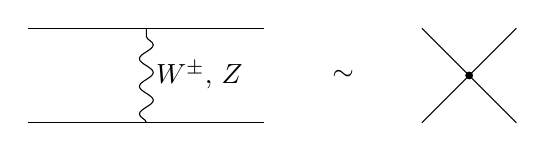
\begin{tikzpicture}
                \draw (0,0) -- (3,0);
                \draw (0,1.2) -- (3,1.2);
                \draw[decorate,decoration=snake] (1.5,0) -- (1.5,1.2) node[midway,right] {\(W^\pm\), \(Z\)};

                \node at (4,0.6) {\(\sim\)};
                
                \draw (5,0) -- (6.2,1.2);
                \draw (6.2,0) -- (5,1.2);
                \fill (5.6,0.6) circle (0.05);
            \end{tikzpicture}
        \end{figure}
        This is radiation dominated, and \(\sigma \sim G_F^2T^2\), so \(\Gamma \sim G_F^2T^5\). Hence we have 
        \begin{equation}
            \frac\Gamma{H} \sim \frac{G_F^2 T^5}{T^2/M_{\text{pl}}} = G_F^2T^3M_{\text{pl}} \sim \left(\frac{T}{\si{\mega\eV}}\right)^3.
        \end{equation}
        So for \(T\lesssim\si{\mega\eV}\), these interactions are not in equilibrium.
\end{itemize}

Non-equlibrium is important. For non-relativistic particles in equilibrium, \(E/T\) is large, and \(E \approx m\), so the average occupancy is
\begin{equation}
    f(p) \sim \frac1{e^{E/T}\pm 1} \to e^{-m/T}.
\end{equation}
This is \emph{Boltzmann equilibrium}. Were the particles to remain in equilibrium, their density would hence decay to zero. When the particles leave equilibrium, the number density of the particles ``freezes out'' to a relic density.
\begin{figure}[H]
    \centering
    \begin{tikzpicture}
        \draw[thick,->] (0,0) -- (10,0) node[right] {\(\displaystyle\frac{m}{T}\)};
        \draw[thick,->] (0,0) -- (0,5) node[above] {\(\displaystyle\frac{n}{T^3}\)};
        \draw (0,4) .. controls (5,4) and (2,1) .. (10,1) node[right] {relic density};
        \draw[thick,<-] (3.5,3.1) -- (4.5,4.1) node[above] {Boltzmann suppression};
        \node[rotate=-7] at (7.5,1.5) {freeze-out};
    \end{tikzpicture}
\end{figure}

We will explore this for:
\begin{itemize}
    \item Dark matter production
    \item BBN
    \item Decoupling and CMB formation
\end{itemize}

\subsection{Equilibrium statistical physics}
Consider a particle with \(g\) internal degrees of freedom in a box of volume \(V=L^3\). The momentum eigenvalues have spacing \(\frac{h}{L}\), so the phase space density of states is given by
\begin{equation}
    g\frac1{L^3}\frac{L^3}{h^3} = \frac{g}{h^3} = \frac{g}{(2\pi)^3},
\end{equation}
where the last equality makes use of \(\hbar = 1\). The distribution function \(f(\vb{x},\vb{p},t)\) tells us how the particle is distributed in the box. We assume that \(f\) is:
\begin{itemize}
    \item Homogeneous (independent of \(\vb{x}\))
    \item Isotropic (only dependent on \(\vb{p}\) through \(p = |\vb{p}|\))
    \item Time-dependent only through dependence on the temperature
\end{itemize}
Hence we can write \(f = f(p)\). The particle number density, mass density and pressure are given by
\begin{align}
    n &= \frac{g}{(2\pi)^3}\int\dd[3]{p}f(p), \\
    \rho &= \frac{g}{(2\pi)^3}\int\dd[3]{p}E(p)f(p), \\
    P &= \frac{g}{(2\pi)^3}\int\dd[3]{p}f(p)\frac{p^2}{3E(p)},
\end{align}
where \(E(p) = \sqrt{p^2+m^2}\).

The distribution function can be found by maximising the entropy. In kinetic equilibrium it is given by
\begin{equation}
    f(p) = \frac1{e^{\frac{E(p)-\mu}{T}}\pm 1},
\end{equation}
where we take \(+\) for fermions, and \(-\) for bosons, and \(\mu\) is the chemical potential (note we take \(k_B=1\)). In thermodynamics we have
\begin{equation}
    \dd{U} = \mu\dd{N} + T\dd{S} - P\dd{V}.
\end{equation}
In general \(\mu = \mu(T)\). In chemical equilibrium, the chemical potentials of the species involved in an interaction must balance; for example if we are looking at \(1+2\leftrightarrow3+4\), then we must have \(\mu_1 + \mu_2 = \mu_3 + \mu_4\). As a consequence, we have for example that the non-conservation of photon number means \(\mu_\gamma=0\).

When a system is in both kinetic equilibrium and chemical equilibrium, it is said to be in \emph{thermal} equilibrium. Any species in thermal equilibrium have the same temperature \(T_i = T\). Also, thermal equilibrium is maintained for \(\Gamma_i \gg H\).

\subsubsection*{Densities}
Set \(\mu = 0\). We have
\begin{align}
    n &= \frac{g}{(2\pi)^3}\int\dd[3]{p}f(p) \\
      &= \frac{g}{2\pi^2}\int_0^\infty \dd{p} p^2 f(p) \\
      &= \frac{g}{2\pi^2}\int_0^\infty \dd{p}\frac{p^2}{e^{E(p)/T}\pm1}.
    \intertext{Define \(x=\frac{m}{T}\) and \(\xi = \frac{P}{T}\). We have:}
    n &= \frac{g}{2\pi^2}T^3\int_0^\infty \dd{\xi}\frac{\xi^2}{e^{\sqrt{\xi^2+x^2}}\pm 1} \\
      &\equiv \frac{g}{2\pi^2}T^3I_\pm(x).
\end{align}
Simliarly, we have
\begin{align}
    \rho &= \frac{g}{(2\pi)^3}\int\dd[3]{p}E(p)f(p) \\
         &= \frac{g}{2\pi^2}\int_0^\infty\dd{p}\frac{p^2\sqrt{p^2+m^2}}{e^{\sqrt{p^2+m^2}/T}\pm1} \\
         &= \frac{g}{2\pi^2}T^4\int^\infty_0\dd{\xi}\frac{\xi^2\sqrt{\xi^2+x^2}}{e^{\sqrt{\xi^2+x^2}}\pm 1} \\
         &\equiv \frac{g}{2\pi^2}T^4J_\pm(x).
\end{align}
These integrals cannot be taken exactly, but we can examine how they behave in certian limits. The following formulas will come in useful:
\begin{equation}
    \int_0^\infty\dd{\xi}\frac{\xi^n}{e^\xi-1} = \zeta(n+1)\Gamma(n+1)
    ,\quad
    \int_0^\infty\dd{\xi}\frac{\xi^n}{e^\xi} = \frac12\Gamma\left(\frac12(n+1)\right)
\end{equation}

Consider first the ultra relativistic limit, \(x\ll 1\). We have 
\begin{equation}
    I_\pm(x \ll 1) \approx I_\pm(0) = \int_0^\infty\dd{\xi}\frac{\xi^2}{e^\xi\pm1}.
\end{equation}
For bosons we just use the first formula above to write
\begin{equation}
    I_-(0) = \zeta(3)\Gamma(3) = 2\zeta(3).
\end{equation}
For fermions we make use of the following trick:
\begin{equation}
    \frac{1}{e^\xi+1} = \frac{1}{e^\xi-1} - 2\frac{1}{e^{2\xi}-1}
\end{equation}
With this, we can write
\begin{align}
    I_+(0) &= \int^\infty_0 \dd{\xi}\frac{\xi^2}{e^\xi+1} \\
           &= I_-(0) - 2\int^\infty_0 \dd{\xi}\frac{\xi^2}{e^{2\xi}-1} \\
           &= I_-(0) - 2\left(\frac12\right)^3I_-(0) \\
           &= \frac{3}{4}I_-(0) = \frac32\zeta(3).
\end{align}
Therefore we have
\begin{equation}
    n = \frac{g \zeta(3)}{\pi^2}T^3 \times 
    \begin{cases}
        1 & \text{bosons}, \\
        \frac{3}{4} & \text{fermions}.
    \end{cases}
\end{equation}

Similarly we have
\begin{align}
    J_-(0) &= \zeta(4) \Gamma(4) = \frac{\pi^4}{15}, \\
    J_+(0) &= \left(1-2\left(\frac12\right)^4\right)J_-(0) = \frac78 J_-(0),
\end{align}
and so
\begin{equation}
    \rho = \frac{g\pi^2}{30}T^4\times
    \begin{cases}
        1 & \text{bosons}, \\
        \frac78 & \text{fermions}.
    \end{cases}
\end{equation}

As an application of these results, we can find the number and energy densities of photons in the CMB. We have \(g = 2\) and \(T = \SI{2.7}{\kelvin}\), and plugging these values in we obtain \(n_{\gamma,0} \approx \SI{410}{\centi\metre^{-3}}\) and \(\rho_{\gamma,0} \approx \SI{4.6e-34}{g.cm^{-3}}\).

Now consider the non-relativistic case with \(x\gg1\). We have
\begin{align}
    I_\pm(x\gg1) &= \int_0^\infty\dd{\xi}\frac{\xi^2}{e^{\sqrt{\xi^2+x^2}}\pm1} \\
                 &\approx \int_0^\infty\dd{\xi}\frac{\xi^2}{e^{\sqrt{\xi^2+x^2}}} \\
                 &\approx \int_0^\infty\dd{\xi}\frac{\xi^2}{e^{x + \frac{\xi^2}{2x}}} \\
                 &= e^{-x}\int_0^\infty\dd{\xi}\xi^2e^{-\xi^2/2x} \\
                 &= \sqrt{\frac{\pi}{2}}x^{\frac32}e^{-x}.
\end{align}
Hence for both bosons and fermions we have \(n = g\left(\frac{mT}{2\pi}\right)^{\frac32}e^{-m/T}\). Since \(E(p)\approx m\), we immediately also have \(\rho \approx m n\) (in the non-relativistic limit).

The radiation energy density is given as the sum of the energy density over all relativistic species:
\begin{equation}
    \rho_r = \sum_{\mathclap{i\,\text{relativistic}}}\rho_i = \frac{\pi^2}{30} g_*(T)T^4
\end{equation}
Here we have defined the \emph{effective degrees of freedom}
\begin{equation}
    g_*(T) = \sum_{\mathclap{i\,\text{bosonic}}}g_i\left(\frac{T_i}{T}\right)^4
    + 7/8 \sum_{\mathclap{i\,\text{fermionic}}}g_i\left(\frac{T_i}{T}\right)^4.
\end{equation}
In general \(T_i\ne T\) for decoupled species, but when all particle species are in thermal equilibrium, we have \(T_i=T\), and we can write
\begin{equation}
    g_* = g_*^{\text{th}} = \sum_{\mathclap{i\,\text{bosonic}}}g_i
    + 7/8 \sum_{\mathclap{i\,\text{fermionic}}}g_i.
\end{equation}
At \(T>\SI{e5}{MeV}\), all standard model particles are in equilibrium and are ultra relativistic, so we can directly calculate \(g_*\). There are 28 degrees of freedom in the bosons (2 for the photon, \(3\times3\) for \(W^\pm,Z\), \(8\times2\) for the gluons, and 1 for the Higgs), and 90 in the fermions (\(6\times2\times3\times2\) for the quarks, \(3\times2\times2\) for the charged leptons, and \(3\times1\times2\) for the neutrinos), so the total effective degrees of freedom is
\begin{equation}
    g_* = g_*^{\text{th}} = 28 + \frac78 \times 90 = 106.25.
\end{equation}

\subsubsection*{Entropy}
In equilibrium and for \(\mu = 0\), it can be shown that \(\pdv{P}{T} = \frac{\rho+P}{T}\). Taking \(\mu=0\), we can rewrite the 2nd law of thermodynamics to obtain
\begin{align}
    \dd{S} &= \frac1{T}(\dd{U}+P\dd{V}) \\
           &= \frac1{T}(\dd{\rho}V + (\rho+P)\dd{V}) \\
           &= \frac1{T}(\dd{((\rho+P)V)} - \dd{P}V) \\
           &= \frac1{T}\left(\dd{((\rho+P)V)} - \frac{\rho+P}{T}V\dd{T}\right) \\
           &= \dd{\left(\frac{\rho+P}{T}V\right)} \\
    \implies S &= \frac{\rho+P}{T}V.
\end{align}
Hence we have
\begin{align}
    \dv{S}{t} &= \frac{\dot\rho+\dot{P}}{T}V + \frac{\rho+P}{T}\dot{V} - \frac{\rho+P}{T^2}V\dot{T} \\
              &= \frac{V}{T}\underbrace{\left(\dot{\rho}+(\rho+P)\frac{\dot{V}}{V}\right)}_{\substack{=0\\\text{(continuity equation)}}} + \frac{V}{T}\underbrace{\left(\dot{P} - \frac{\rho+P}{T}\dot{T}\right)}_{=0} = 0,
\end{align}
i.e.\ entropy is conserved in equilibrium. Entropies are seperately conserved for decoupled species. Entropy production requires non-adiabatic processes (e.g. 1st order phase transitions, or out of equilibrium particle decay. We define the \emph{entropy density} as \(s = \frac{S}{V} = \frac{\rho+P}{T}\). For a collection of species we have
\begin{equation}
    s = \sum_i \frac{\rho_i+P_i}{T_i} = \frac{2\pi^2}{45}g_{*s}(T) T^3,
\end{equation}
which defines \(g_{*s}\), the \emph{effective degrees of freedom in entropy}. If we split this between the degrees of freedom of those species in equilibrium and those that have decoupled, writing \(g_{*s} = g_{*s}^{\text{th}} + g_{*s}^{\text{dec}}\), then it is true that \(g_{*s}^{\text{th}} = g_*^{\text{th}}\), but \(g_{*s}^{\text{dec}}\ne g_*^{\text{dec}}\), due to differing powers of \(T\):
\begin{equation}
    g_{*s}^{\text{dec}} = \sum_{\mathclap{i\,\text{bosonic}}}g_i\left(\frac{T_i}{T}\right)^3
    + 7/8 \sum_{\mathclap{i\,\text{fermionic}}}g_i\left(\frac{T_i}{T}\right)^3
\end{equation}
Conservation of entropy provides us with \(s\sim a^{-3}\), so
\begin{equation}
    a^3s \sim a^3g_{*s}(T)T^3 \sim \text{constant}.
\end{equation}
If we define \(N_i = \frac{n_i}{s}\), then \(N_i\sim\text{constant}\) if there is no particle production. Also, we have
\begin{equation}
    T \sim a^{-1}g_{*s}^{-\frac13}(T).
\end{equation}
If we plug in actual values then we can obtain the following useful approximation:
\begin{equation}
    \frac{T}{\SI{1}{MeV}} \approx 1.5 g_*^{-\frac14} \left(\frac{\SI{1}{s}}{t}\right)^{\frac12}
\end{equation}

\subsubsection*{Neutrino decoupling}
Neutrinos couple to the thermal bath through the weak interactions. For these interactions we have \(\sigma \sim G_F^2T^2\), where \(G_F\sim \SI{e-5}{GeV^2}\). \(n\sim T^3\) and \(H\sim \frac{T^2}{M_{\text{pl}}}\), so
\begin{equation}
    \frac{\Gamma}{H} = \frac{n\sigma v}{H} \sim \frac{G_F^2T^5}{T^2/M_{\text{pl}}} \sim \left(\frac{T}{\SI{1}{MeV}}\right)^3.
\end{equation}
Hence for \(T\lesssim \SI{1}{MeV}\) we see that neutrinos decouple. At decoupling \(T_\nu = T_\gamma\).

Soon after neutrino decoupling, \(e^+\) and \(e^-\) annihilate, and their energy and entropy are transferred only to the photons.

Our aim is to calculate \(\left.\frac{T_\nu}{T_\gamma}\right|_{\text{after}}\). We can write
\begin{equation}
    \left.T_\gamma\right|_{\text{before}} \left.a\right|_{\text{before}} =
    \left.T_\nu\right|_{\text{before}} \left.a\right|_{\text{before}} =
    \left.T_\nu\right|_{\text{after}} \left.a\right|_{\text{after}} ,
\end{equation}
where the second equality follows from the fact that \(\nu\) are free streaming. Also, conservation of entropy gives
\begin{equation}
    \left[g_{*s}^{\text{th}}(T_\gamma a)^3\right]_{\text{before}} = 
    \left[g_{*s}^{\text{th}}(T_\gamma a)^3\right]_{\text{after}}.
\end{equation}
We are only concerned with the photons and electrons/positrons. Before, we have \(g_{*s}^{\text{th}} = 2 + \frac78(2\times2) = \frac{11}2\). Afterwards, entropy has been transferred from \(e^\pm\) to \(\gamma\), so \(g_{*s}^{\text{th}} = 2\). Combining everything we find
\begin{equation}
    \frac{11}2\left(\left.T_\nu\right|_{\text{after}}\right)^3
    =
    2\left(\left.T_\nu\right|_{\text{before}}\right)^3 
    \implies
    \left.\frac{T_\nu}{T_\gamma}\right|_{\text{after}} = \left(\frac4{11}\right)^{\frac13}.
\end{equation}

\subsection{Beyond equilibrium}
\subsubsection*{Boltzmann equation}
With no interactions we have
\begin{equation}
    \dv{n_i}{t} + 3\frac{\dot{a}}{a} n_i = 0.
\end{equation}
The Boltzmann equation generalises this:
\begin{equation}
    \frac1{a^3}\dv{(n_ia^3)}{t} = \underbrace{C_i(\{n_i\})}_{\mathclap{\text{collision term}}}
\end{equation}

Consider an interaction of the form \(1+2\leftrightarrow3+4\). We guess the form of \(C_i\), and write the Boltzmann equation as
\begin{equation}
    \frac1{a^3}\dv{(n_1a^3)}{t} = - \underbrace{\alpha n_1 n_2}_{\mathclap{\text{destruction rate}}} + \overbrace{\beta n_3 n_4}^{\mathclap{\text{production rate}}},
\end{equation}
where \(\alpha = \expval{\sigma v}\) is the \emph{thermally averaged cross-section}. The interaction rate of species 1 is \(\Gamma_1 = n_2\alpha\). \(n_2\) is cosmology dependent, and \(\alpha\) is particle physics dependent.

What about \(\beta\)? In equilibrium, the collision term should vanish, so we write \(\beta = \left(\frac{n_1n_2}{n_3n_4}\right)_{\text{eq}}\alpha\). Hence, the Boltzmann equation is
\begin{equation}
    \frac1{a^3}\dv{(a^3n_1)}{t} = - \expval{\sigma v}\left(n_1n_2 - \left(\frac{n_1n_2}{n_3n_4}\right)_{\text{eq}} n_3n_4\right).
\end{equation}
We can rewrite this in terms of \(N_i = \frac{n_i}{s}\) to obtain
\begin{equation}
    \frac1{a^3}\dv{(a^3N_1s)}{t} = - \expval{\sigma v}s^2\left(N_1N_2 - \left(\frac{N_1N_2}{N_3N_4}\right)_{\text{eq}} N_3N_4\right).
\end{equation}
Since \(a^3s\) is constant, we can hence write
\begin{equation}
    \dv{N_1}{t} = - \underbrace{\expval{\sigma v}sN_2}_{=\Gamma_1}\left(N_1 - \left(\frac{N_1N_2}{N_3N_4}\right)_{\text{eq}} \frac{N_3N_4}{N_2}\right).
\end{equation}
We can rewrite this again to obtain
\begin{equation}
    \dv{\log N_1}{\log a} = - \frac{\Gamma_1}{H}\left(1 - \left(\frac{N_1N_2}{N_3N_4}\right)_{\text{eq}}\frac{N_3N_4}{N_1N_2}\right).
\end{equation}
From this we see for \(\frac{\Gamma_1}{H}\gg1\), densities are quickly pushed to equilibrium, but for \(\frac{\Gamma_1}{H}\ll 1\), \(N_1 \to \text{constant}\) (this is freezeout).

\subsubsection*{Dark Matter}
There are several candidates for dark matter. The first type is known as ``hot dark matter'', because it would have been relativistic at decoupling. This would be \(\nu\) in the standard model, but unfortunately this doesn't work, as it would have led to an erasure of structure in the universe. The second type is ``cold dark matter'', non-relativistic at decoupling. We will focus on one type of CDM, known as WIMPs (weakly interacting massive particles).

We will use \(X\) to denote the WIMP, and assume that they are coupled to some strongly interacting particle \(l\) (e.g.\ charged leptons) via the interaction \(X+\bar{X} \leftrightarrow l + \bar{l}\). We assume that \(n_l\approx n_l^{\text{eq}}\), and \(n_X = n_{\bar{X}}\) initially. The Boltzmann equation then reads
\begin{equation}
    \dv{N_X}{t} = -\expval{\sigma v}s(N_X^2 - (N_X^{\text{eq}})^2).
\end{equation}
If we define \(x = \frac{m_X}{T}\), then we have \(\dv{t} = \dot{x}\dv{x} = -x\frac{\dot{T}}{T}\dv{x} = xH\dv{x}\), so we can write this as
\begin{equation}
    xH\dv{N_X}{x} = -\expval{\sigma v}s(N_X^2 - (N_X^{\text{eq}})^2).
\end{equation}
During radiation domination, \(H\sim T^2\), so \(H(x) = H(m_X)\frac1{x}\), and hence
\begin{equation}
    \frac{H(m_X)}{x}\dv{N_X}{x} = -\expval{\sigma v}s(N_X^2 - (N_X^{\text{eq}})^2).
\end{equation}
Now, subsituting in \(s = \frac{2\pi^2}{45}g_{*s}(T)m_X^3\frac{1}{x^3}\), we obtain the \emph{Riccati equation}
\begin{equation}
    \dv{N_x}{x} = -\frac\lambda{x^2}\left(N_X^2-(N_X^{\text{eq}})^2\right),
\end{equation}
where \(\lambda = \frac{\expval{\sigma v}}{H(m_X)} \frac{2\pi^2}{45} g_{*s}(x)m_X^3\). Typically \(\lambda \gg 1\), and it is often a good approximation to take \(\lambda \approx \text{constant}\).

To find an approximate solution, we assume that freezeout occurs at \(x=x_f\), and that \(N_X^{\text{eq}}(x) \ll N_X(x)\) for \(x > x_f\). Then in this region we have
\begin{align}
    \dv{N_X}{x} &= -\frac\lambda{x^2}N_X^2 \\
    \implies \dv{x} \left(\frac1{N_X}\right) &= \frac{\lambda}{x^2} \\
    \implies \frac1{N_X^\infty} - \frac1{N_X(x_f)} &= \frac\lambda{x_f}.
\end{align}
If we assume \(N_X(x_f)\gg N_X^\infty\), then we can deduce that \(N_X^\infty \approx \frac{x_f}{\lambda}\). We can estimate \(x_f\) by using \(\Gamma(x_f) = H(x_f)\).

We wish to estimate the dark matter density today. We have
\begin{equation}
    \Omega_X = \frac{\rho_{X,0}}{\rho_{\text{crit},0}} 
             = \frac{m_Xn_{X,0}}{3M_{\text{pl}}^2H_0^2} 
             = \frac{m_XN_{X,0}s_0}{3M_{\text{pl}}^2H_0^2}
\end{equation}
If we assume that WIMP freezeout occured in the distant past, we can assume \(N^0_X \approx N^\infty_X\), and hence
\begin{equation}
    \Omega_X = \frac{x_f}{\lambda}m_X\frac{s_0}{3M_{\text{pl}}^2H_0^2} = m_Xx_f \frac{g_{*s}(T_0)T_0^3}{\expval{\sigma v}g_{*s}(m_X)} \frac{H(m_X)}{m_X^3}\frac1{3M_{\text{pl}}^2H_0^2}.
\end{equation}
Note that
\begin{equation}
    H(m_X) = \left(\frac{\rho_r}{3M_{\text{pl}}^2}\right)^{\frac12} \approx \frac\pi3 \left(\frac{g_*(m_X)}{10}\right)^{\frac12} \frac{m_X^2}{M_{\text{pl}}},
\end{equation}
so we have
\begin{equation}
    \Omega_X = \frac\pi9\frac{x_f}{\expval{\sigma v}} \left(\frac{f_*(m_X)}{10}\right)^{\frac12} \frac{g_{*s}(T_0)}{g_{*s}(m_X)} \frac{T_0^3}{3M_{\text{pl}}^2H_0^2}.
\end{equation}
Assuming that \(g_{*s}(m_X) \approx g_*(m_X)\) and substituting in appropriate values, this is
\begin{equation}
    \Omega_Xh^2 \approx 0.1 \left(\frac{x_f}{10}\right)\left(\frac{10}{g_*(m_X)}\right)^{\frac12}\frac{\SI{e-8}{GeV^{-2}}}{\expval{\sigma v}}.
\end{equation}
This replicates the observed dark matter density if \(\sqrt{\expval{\sigma v}} \sim \SI{e-4}{GeV^{-1}}\approx 0.1 \sqrt{G_F}\). This correspondence is known as the WIMP miracle. (Some people believe that it goes some way towards solving the hierarchy problem.)

\subsubsection*{Recombination}
Above \(T\approx\SI{1}{eV}\), photons and electrons are in equilibrium through \(e^- + p^+ \leftrightarrow H + \gamma\). At the relevant temperatures, \(e^-\), \(p^+\) and \(H\) are non-relativistic, so we have
\begin{equation}
    n_i^{\text{eq}} = g_i\left(\frac{m_i T}{2\pi}\right)^{\frac32}e^{-\frac{m_i-\mu_i}{T}} \qq{for} i \in \{e^-,p^+,H\}.
\end{equation}
We use the equilibrium condition \(\mu_{e^-} + \mu_{p^+} = \mu_H\) to eliminate the chemical potentials, obtaining
\begin{equation}
    \left(\frac{n_H}{n_en_p}\right)_{\text{eq}} = \frac{g_H}{g_eg_p} \left(\frac{m_H}{m_em_p}\frac{2\pi}{T}\right)^{\frac32} e^{(m_e+m_p-m_H)/T}.
\end{equation}
Note that the binding energy of hydrogen is \(B_H = m_e+m_p-m_H \approx \SI{13.6}{eV}\). Also, we have \(g_H=4\) and \(g_e = g_p = 2\). Additionally we assume charge neutrality, so that \(n_e = n_p\). Using \(m_p/m_H\approx 1\), we hence have
\begin{equation}
    \left(\frac{n_H}{n_e^2}\right)_{\text{eq}} = \left(\frac{2\pi}{m_e T}\right)^{\frac32} e^{B_H/T}.
\end{equation}
The \emph{free electron fraction} is defined to be \(X_e = \frac{n_e}{n_b} \approx \frac{n_e}{n_p+n_H}\) (\(n_b\) is the baryon density). We also define the ``baryon to photon ratio'' \(\eta = \frac{n_b}{n_\gamma}\). Note that
\begin{equation}
    \frac{n_H}{n_e^2} = \frac{n_b-n_e}{n_e^2} = \frac1{n_b}\frac{1-X_e}{X_e^2},
\end{equation}
so we can write 
\begin{equation}
    \frac{1-X_e}{X_e^2} = n_b \frac{n_H}{n_e^2} = \eta n_\gamma \frac{n_H}{n_e^2},
\end{equation}
and hence
\begin{equation}
    \left(\frac{1-X_e}{X_e^2}\right)_{\text{eq}} = \frac{2\zeta(3)}{\pi^2}\eta\left(\frac{2\pi T}{m_e}\right)^{\frac32} e^{B_H/T}.
\end{equation}
This is the \emph{Saha equation}. The smallness of \(\eta \sim 10^{-9}\) suppresses recombination until \(T\ll B_H\) -- this is the first surprise: recombination is ``late''. The second surprise is that recombination happens very suddently: at \(T\approx \SI{0.3}{eV}\), \(X_e=0.1\), and at \(T\approx \SI{0.35}{eV}\), \(X_e = 0.9\). We will take the time of recombination to be at \(X_{\text{rec}} = 0.1\), \(T_{\text{rec}}=\SI{0.3}{eV}\), \(Z_{\text{rec}} \approx 1270\), \(t_{\text{rec}} \approx \SI{290000}{yrs}\).

Soon after recombination, photons decouple from the electrons. Thompson scattering has been keeping the two species in equilibrium, and occurs with the rate \(\Gamma_\gamma = n_e\sigma_{\text{Th}}\), where
\begin{equation}
    \sigma_{\text{Th}} = \frac{8\pi}{3}\frac{\alpha_e^2}{m_e^2} \approx \SI{2e-3}{MeV^{-2}}.
\end{equation}
Decoupling occurs when \(\Gamma_\gamma = H\), so
\begin{equation}
    n_b(T_{\text{dec}})X_e(T_{\text{dec}})\sigma_{\text{Th}} \approx H_0\sqrt{\Omega_m} \left(\frac{T_{\text{dec}}}{T_0}\right)^{\frac32}.
\end{equation}
Using the Saha equation leads to \(T_{\text{dec}} \approx \SI{0.27}{eV}\), \(X_e(T_{\text{dec}}) \approx 0.01\), \(Z_{\text{dec}} = 1100\), \(t_{\text{dec}} = \SI{380000}{yrs}\).

Note that decoupling leads to the birth of the CMB.

\subsubsection*{Big Bang nucleosynthesis}
Light elements such as H, He, and Li were synthesised during the Big Bang. The goal in this section is to determine why we observe \(Y_p \equiv \frac{n_{\text{He}}}{n_{\text{H}}} = \frac1{16}\). To explain this, we must carry out a calculation of several steps.

\begin{figure}[H]
    \centering
    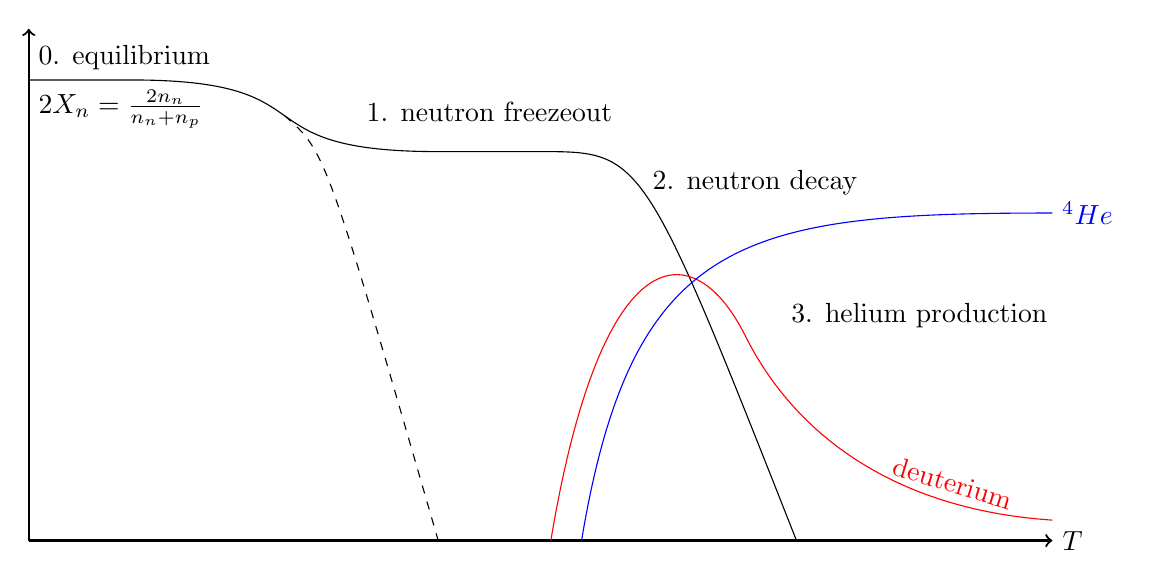
\begin{tikzpicture}[scale=1.3]
        \draw[thick,->] (0,0) -- (10,0) node[right] {\(T\)};
        \draw[thick,->] (0,0) -- (0,5);
        \draw[dashed] (2.5,4.15) .. controls (2.9,3.8) .. (4,0);
        \draw (0,4.5) -- (1,4.5) .. controls (3,4.5) and (2,3.8) .. (4,3.8) -- (5,3.8) .. controls (6,3.8) .. (7.5,0);
        \draw[red] (5.1,0) .. controls (5.6,3) and (6.5,3) .. (7,2) .. controls (7.5,1) and (8.5,0.3) .. (10,0.2) node[above,sloped,near end] {deuterium};
        \draw[blue] (5.4,0) .. controls (5.9,3) and (7,3.2) .. (10,3.2) node[right] {\({}^4\text{He}\)};
        \node[below right] at (0,4.5) {\(2X_n = \frac{2n_n}{n_n+n_p}\)};
        \node[above right] at (0,4.5) {0. equilibrium};
        \node[above] at (4.5,4) {1. neutron freezeout};
        \node[right] at (6,3.5) {2. neutron decay};
        \node at (8.7,2.2) {3. helium production};
    \end{tikzpicture}
\end{figure}

\begin{enumerate}
    \setcounter{enumi}{-1}
    \item First we must consider equilibrium densities.

        Equilibrium between neutrons and protons is maintained by weak interactions like \(n+\nu_e \leftrightarrow p + e^-\). We assume that \(\mu_{\nu_e},\mu_e \ll 1\) so that \(\mu_n \approx \mu_p\), and hence 
        \begin{equation}
            \left(\frac{n_n}{n_p}\right)_{\text{eq}} = \underbrace{\frac{g_n}{g_p}}_{=1}\underbrace{\left(\frac{m_n}{m_p}\right)^{\frac32}}_{\approx 1} e^{-(m_n-m_p)/T} \approx e^{-Q/T},
        \end{equation}
        where \(Q = m_n-m_p \approx \SI{1.3}{MeV}\).

        Deuterium (\(D=p^+n={}^2H^+\)) is generated during BBN, and it will be useful to determine the equilibrium Deuterium fraction. This equilibrium is maintained by \(n+p\leftrightarrow D+\gamma\), so we have \(\mu_n+\mu_p=\mu_D\), and can write
        \begin{equation}
            \left(\frac{n_D}{n_nn_p}\right)_{\text{eq}} = \frac{g_D}{g_ng_p}\left(\frac{m_D}{m_nm_p}\frac{2\pi}{T}\right)^{\frac32}\exp[-(m_d-m_n-m_p)/T] \approx \frac34\left(\frac2{m_p}\frac{2\pi}T\right)^{\frac32}e^{B_D/T},
        \end{equation}
        where we have used \(g_D=3\), \(g_n=g_p=2\), \(m_D\approx 2m_n\) and set \(B_d = m_n+m_p - m_D \approx \SI{2.2}{MeV}\). Now we use
        \begin{equation}
            n_n \sim n_b = \eta n_\gamma = \eta \frac{2\zeta(3)}{\pi^2}T^3
        \end{equation}
        to obtain the order of magnitude estimate
        \begin{equation}
            \left(\frac{n_D}{n_p}\right)_{\text{eq}} \sim \eta \left(\frac{T}{m_p}\right)^{\frac32} e^{\frac{B_D}{T}}.
        \end{equation}
    \item Weak interactions freeze out when neutrinos decouple, at around \(T = T_{\nu_{\text{dec}}}\sim \SI{0.8}{MeV}\). We have
        \begin{equation}
            X_n = \frac{n_n}{n_n+n_p} \implies X_n^{\text{eq}} = \frac{e^{-Q/T}}{1 + e^{-Q/T}},
        \end{equation}
        and plugging in the various values, we get \(X_n^{\text{eq}}(T_{\nu_{\text{dec}}}) \approx 0.17 \approx \frac16\). Hence, we approximate \(X_n^\infty \approx \frac16\).
    \item Neutrons have a decay lifetime of \(\tau_n = \SI{886.7\pm0.8}{s} \sim \SI{900}{s}\). The decay produces a proton by \(n \to p + e^- + \bar\nu_e\). Thus we set 
        \begin{equation}
            X_n(t) \approx \frac16 e^{-t/\tau_n},
        \end{equation}
        where \(t\) is time after neutron freezeout.
    \item Helium can't form directly from neutrons and protons because densities are too low. Instead we must go through deuterium (this forms a so-called ``deuterium bottleneck''). We first have
        \begin{equation}
            n + p^+ \to D^+ + \gamma,
        \end{equation}
        and then
        \begin{align}
            D + p^+ &\to {}^3\text{He} + \gamma, \\
            D + {}^3\text{He} &\to {}^4\text{He} + p^+.
        \end{align}
        We will assume that \(n_D \approx n_D^{\text{eq}}\). We want a rough estimate for when deuterium is produced in sufficient numbers that He forms. To find this we set \(\left(\frac{n_D}{n_p}\right)_{\text{eq}}\approx1\) to obtain \(T_{\text{nuc}} \sim \SI{0.06}{MeV}\) and \(t_{\text{nuc}} \sim \SI{300}{s}\). Hence we find \(X_n(t_{\text{nuc}}) \sim \frac16e^{-\frac{300}{900}} \sim \frac18\).

        Virtually all neutrons fuse into \({}^4\text{He}\), so we can write \(n_{\text{He}} = \frac12n_n(t_{\text{nuc}})\), and thus we have
        \begin{equation}
            \frac{n_{\text{He}}}{n_{\text{H}}} = \frac{n_{\text{He}}}{n_p} \approx \frac{\frac12 X_n(t_{\text{nuc}})}{1 - X_n(t_{\text{nuc}})} \approx \frac12 X_n(t_{\text{nuc}}) \sim \frac1{16}.
        \end{equation}
        Hence we obtain the desired result.
\end{enumerate}

\section{Quantum origin of density perturbations}
\subsection{Classical evolution of perturbations}
Consider the action of spacetime, including the inflaton:
\begin{equation}
    S = \int\dd[4]{x} \sqrt{-g}\left(\frac{M_{\text{pl}}^2}2 R - \frac12 \partial_\mu\phi\partial^\mu\phi - V(\phi)\right)
\end{equation}
We get the equations of motion by setting \(\delta S = 0\) when we vary the free variables. If we vary \(g_{\mu\nu}\), we recover Einstein's equations. If we vary \(\phi\), we have
\begin{align}
    \delta S &= \int\dd[4]{x}\sqrt{-g}\left(-\partial_\mu\delta\phi\partial^\mu\phi - \delta\phi\partial_\phi V\right) \\
             &= \int\dd[4]{x} \left[\delta\phi\partial_\mu\left(\sqrt{-g}\partial^\mu\phi\right) - \delta\phi \partial_\phi V \sqrt{-g}\right] \\
             &= \int\dd[4]{x} \sqrt{-g}\left[\delta\phi\left(\frac1{\sqrt{-g}}\delta_\mu\left(\sqrt{-g}\partial^\mu\phi\right)-\partial_\phi V\right)\right].
\end{align}
Define \(\dalembertian = \frac1{\sqrt{-g}}\partial_\mu(\sqrt{-g}g^{\mu\nu}\partial_\mu)\), the \emph{covariant d'Alembertian}. Then we obtain the Klein-Gordon equation
\begin{equation}
    \dalembertian\,\phi - \partial_\phi V = 0.
\end{equation}
In an unperturbed FLRW universe, we showed before that this becomes
\begin{equation}
    \phi'' + 2\mathcal{H}\phi' - \nabla^2\phi + a^2\partial_\phi V = 0.
\end{equation}
To find a classical equation of motion for perturbations \(\delta\phi\), we vary the Klein-Gordon equation, obtaining
\begin{equation}
    (\delta\dalembertian)\bar\phi + \dalembertian\,\delta\phi - \delta\phi\partial^2_\phi V(\bar{\phi}) = 0.
\end{equation}
In the spatially flat gauge, \((\delta\dalembertian)\bar\phi\) is slow-roll suppressed, so we will assume it is 0 for now and take \(g = \bar{g}\). The equation for the perturbations hence becomes
\begin{equation}
    \delta\phi'' + 2\mathcal{H}\delta\phi' - \nabla^2\delta\phi + a^2\delta\phi\partial^2_\phi V(\bar\phi) = 0.
\end{equation}
Now we substitute \(\delta\phi = \frac{f(\vb{x},t)}{a(t)}\). We have \(\delta\phi' = \frac1a f'-\frac1a \mathcal{H}f\) and \(\delta\phi'' = \frac1a\left(f'' - 2\mathcal{H}f' - \frac{a''}{a}f + 2\mathcal{H}^2f\right)\), and substituting these in we obtain
\begin{equation}
    f'' - \frac{a''}a f - \nabla^2 f + a^2 \partial_\phi^2V(\bar\phi)f = 0.
\end{equation}
Under the slow-roll approximation, we have
\begin{equation}
    \frac{\partial_\phi^2 V}{H^2} \approx \frac{3M_{\text{pl}}^2\partial^2_{\phi}V}{V} = 3\eta_V \ll 1,
\end{equation}
so \(a^2\partial_\phi^2V \ll H^2a^2 = \mathcal{H}^2\).
Also, during inflation \(H\) is constant, and we have \(a' = a^2H\), \(a'' = 2 a'aH\), and hence
\begin{equation}
    \frac{a''}{a} = 2a'H = 2a^2H^2 = 2\mathcal{H}^2.
\end{equation}
Therefore we can ignore the \(a^2\partial^2_\phi V\) term, and doing so we obtain
\begin{equation}
    f'' - \nabla^2 f - \frac{a''}{a}f = 0.
\end{equation}
This is known as the \emph{Mukhanov-Sasaki equation}. For a plane wave \(f(\tau,\vb{x}) = e^{i\vb{k}\vdot\vb{x}}f_{\vb{k}}(\tau)\), this takes the form
\begin{equation}
    f_{\vb{k}}'' + \left(|\vb{k}|^2 - \frac{a''}{a}\right)f_{\vb{k}} = 0,
\end{equation}
and on subhorizon scales, \(\frac{a''}{a} = 2\mathcal{H}^2 \ll |\vb{k}|^2\), so we have
\begin{equation}
    f_{\vb{k}}'' + |\vb{k}|^2f_{\vb{k}} = 0.
\end{equation}
This is a simple harmonic oscillator. Quantum fluctuations originate from zero point fluctutations of the SHO.

\subsection{Quantum Oscillators}
Consider a 1D quantum mechanical simple harmonic oscillator. Using \(q\) as a coordinate and using unit mass, we have Lagrangian
\begin{equation}
    L = \frac12\dot{q}^2 - \frac12\tilde{k}q^2.
\end{equation}
The Euler-Lagrange equation implies \(\ddot{q} + \tilde{k}q = 0\), which permits solutions of the form \(q(t) = Ae^{\pm i\omega t}\), where \(\omega^2 = \tilde{k}\). The momentum conjugate to \(q\) is \(p = \pdv{L}{\dot{q}} = \dot{q}\), and we have Hamiltonian \(H(p,q) = \frac12p^2 + \frac12\omega^2q^2\).

Under canonical quantisation, we promote \(q\) and \(p\) to time dependent operators \(\hat{q}(t)\) and \(\hat{p}(t)\) (Heisenberg picture), and impose the relation \([\hat{q}(t),\hat{p}(t)] = i\) (using \(\hbar = 1\)).

We perform a ``mode expansion'', writing
\begin{align}
    \hat{q}(t) &= q(t)\hat{a} + q^*(t)\hat{a}^\dagger, \\
    \hat{p}(t) &= \dot{q}(t)\hat{a} + \dot{q}^*(t)\hat{a}^\dagger.
\end{align}
\(q(t)\) is the mode function, satisfying \(\ddot{q} = -\omega^2q\), i.e.\ \(q=Ae^{\pm i\omega t}\). Substituting this into the commutation relation above, we obtain
\begin{equation}
    [\hat{q},\hat{p}] = iW(q,q^*)[\hat{a},\hat{a}^\dagger] = i,
\end{equation}
where \(W(q,q^*) = q\dot{q}^* - \dot{q}q^*\) is the Wronskian. We have some freedom of normalisation here, so we set \(W(q,q^*) = 1\). This is equivalent to choosing ``positive frequency solutions'' so that \(q(t) = \frac1{\sqrt{2\omega}}e^{-i\omega t}\). 

We define the vacuum by \(\hat{a}\ket{0} = 0\) and \(\braket{0}{0}=1\). We have
\begin{equation}
    \langle\hat{H}\rangle = \mel{0}{\hat{H}}{0} = \frac12 \omega.
\end{equation}
Also note that
\begin{equation}
    \expval{\hat{q}} = 0 \qq{and} \langle|\hat{q}|^2\rangle = |q|^2 = \frac1{2\omega}.
\end{equation}

\subsection{Quantum fluctuations in dS}
During slow-roll inflation, expansion is approximately de Sitter (except that it ends), with \(H=\text{constant}\) and \(a(t) = e^{Ht}\), \(\mathcal{H}(\tau) = -\frac1\tau\) (which is greater than 0 as we are taking \(\tau \to 0\) as \(t \to \infty\), giving \(\tau < 0\)). The Mukhanov-Sasaki equation in Fourier space becomes
\begin{equation}
    f''_{\vb{k}} + \underbrace{\left(|\vb{k}|^2-\frac2{\tau^2}\right)}_{\equiv\omega_k^2(\tau)} = 0.
\end{equation}
The classical solution of this goes like:
\begin{itemize}
    \item For subhorizon modes \(|\vb{k}|^2 \gg \frac2{\tau^2}\), so we just have a simple harmonic oscillator.
    \item For superhorizon modes \(|\vb{k}|^2 \ll \frac2{\tau^2}\), the equation becomes \(f''_{\vb{k}} = \frac2{\tau^2}f_{\vb{k}}(\tau) = 0\), with solution
        \begin{equation}
            f_{\vb{k}} = \underbrace{\alpha\tau^{-1}}_{\mathclap{\text{growing}}} + \overbrace{\beta\tau^2}^{\mathclap{\text{decaying}}} \quad \text{(note \(\tau \to 0\)).}
        \end{equation}
\end{itemize}

The conjugate momentum is \(\pi(\vb{x},\tau) = \fdv{\mathcal{L}}{f'} = f'(\vb{x},\tau)\). Now quantise as before, promoting \(f,\pi\) to operators \(\hat{f},\hat{\pi}\), and imposing
\begin{equation}
    [\hat{f}(\vb{x},\tau),\hat{\pi}(\vb{x}',\tau)] = i\delta^{(3)}(\vb{x}-\vb{x}').
\end{equation}
In Fourier space, this is
\begin{equation}
    [\hat{f}_{\vb{k}}(\tau),\hat{\pi}_{\vb{k}}(\tau)] = \int\frac{\dd[3]{x}\dd[3]{x'}}{(2\pi)^3}e^{-i\vb{k}\vdot\vb{x}-i\vb{k}'\vdot\vb{x}'}(i\delta^{(3)}(\vb{x}-\vb{x}')) = \int\frac{\dd[3]{x}}{(2\pi)^3}e^{-i(\vb{k}+\vb{k}')\vdot\vb{x}} = i\delta^{(3)}(\vb{k}+\vb{k}').
\end{equation}
As before, we do a mode expansion for the operators, writing
\begin{align}
    \hat{f}_{\vb{k}}(\tau) &= f_{\vb{k}}(\tau)\hat{a}_{\vb{k}} + f^*_{\vb{k}}(\tau)\hat{a}^\dagger_{\vb{k}}, \\
    \hat{\pi}_{\vb{k}}(\tau) &= f'_{\vb{k}}(\tau)\hat{a}_{\vb{k}} + f^{'*}_{\vb{k}}(\tau)\hat{a}^\dagger_{\vb{k}}.
\end{align}
We have
\begin{equation}
    i\delta^{(3)}(\vb{k}+\vb{k}') = [\hat{f}_{\vb{k}}(\tau),\hat{\pi}_{\vb{k}'}(\tau)] = iW(f_{\vb{k}},f_{\vb{k}'})[\hat{a}_{\vb{k}},\hat{a}^\dagger_{\vb{k}'}].
\end{equation}
To normalise, we set the Wronskian equal to 1, and
\begin{equation}
    [\hat{a}_{\vb{k}},\hat{a}^\dagger_{\vb{k}'}] = \delta^{(3)}(\vb{k}+\vb{k}').
\end{equation}

The vacuum must satisfy \(\hat{a}_{\vb{k}}\ket{0}\) for all \(\vb{k}\) and \(\braket{0}{0}=1\). We need to fix \(f_{\vb{k}}\) in order to fully determine \(\ket{0}\) and \(\hat{a}_{\vb{k}}\). We do this by observing that at early times, modes are deep within the horizon, obeying \(f'' +k^2f=0\). Therefore we match at early times to the modes of a simple harmonic oscillator by enforcing the \emph{Bunch-Davies initial condition}
\begin{equation}
    \lim_{\tau\to-\infty}f_{\vb{k}}(\tau) = \frac1{\sqrt{2k}}e^{-ik\tau}.
\end{equation}
In dS, the M-S equation has the unique solution
\begin{equation}
    f_{\vb{k}}(\tau) = \alpha\frac{e^{-ik\tau}}{\sqrt{2k}}\left(1-\frac{i}{k\tau}\right) + \beta\frac{e^{+ik\tau}}{\sqrt{2k}}\left(1+\frac{i}{k\tau}\right).
\end{equation}
Using the Bunch-Davies initial condition, we set \(\alpha=1\) and \(\beta=0\). Thus we obtain the \emph{Bunch-Davies mode function}
\begin{equation}
    f_{\vb{k}}(\tau) = \frac{e^{-ik\tau}}{\sqrt{2k}}\left(1-\frac{i}{k\tau}\right).
\end{equation}
Now we can compute the variance of 
\begin{equation}
    \hat{f}(\tau,\vb{x}) = \int\frac{\dd[3]{k}}{(2\pi)^{\frac32}}e^{i\vb{k}\vdot\vb{x}}\left[f_{\vb{k}}(\tau)\hat{a}_{\vb{k}} + f^*_{\vb{k}}(\tau)\hat{a}^\dagger_{\vb{k}}\right].
\end{equation}
\begin{align}
    \langle|\hat{f}|^2\rangle &= \mel{0}{\hat{f}(\tau,0)\hat{f}(\tau,0)}{0} \\
                              &= \int\frac{\dd[3]{k}\dd[3]{k'}}{(2\pi)^3}e^{i(\vb{k}+\vb{k}')\vdot\vb{0}} \mel{0}{(f_{\vb{k}}\hat{a}_{\vb{k}} + f^*_{\vb{k}}\hat{a}^\dagger_{\vb{k}})(f_{\vb{k}'}\hat{a}_{\vb{k}'} + f^*_{\vb{k}'}\hat{a}^\dagger_{\vb{k}'})}{0} \\
                              &= \int\frac{\dd[3]{k}\dd[3]{k'}}{(2\pi)^3}f_{\vb{k}}f_{\vb{k}'}^*\underbrace{\mel{0}{\hat{a}_{\vb{k}}\hat{a}^\dagger_{\vb{k}'}}{0}}_{=\delta^{(3)}(\vb{k}+\vb{k}')} \\
                              &= \int\frac{\dd[3]{k}}{(2\pi)^3} |f_{\vb{k}}|^2 \\
                              &= \frac{4\pi}{(2\pi)^3}\int\dd{k}k^2|f_k|^2 \\
                              &= \int\dd{\log k}\Delta^2_f(k,\tau) \qq{where} \Delta^2_f(k,\tau) = \frac1{2\pi^2}k^3|f_k|^2.
\end{align}
\(\Delta^2_f(k,\tau)\) is the power spectrum of \(f\). We can find the power spectrum of the perturbations by dividing by \(a^2\):
\begin{align}
    \Delta^2_{\delta\phi}(k,\tau) &= \frac{1}{2\pi^2}k^3\frac{|f_k|^2}{a^2} \\
                                  &= \frac1{a^2}\left(\frac{k}{2\pi}\right)^2\left(1+\frac1{(k\tau)^2}\right) \\
                                  &= \left(\frac{H}{2\pi}\right)^2\left(1+\left(\frac{k}{aH}\right)^2\right)
\end{align}
For superhorizon modes \(k \gg aH\), this is \(\approx \left(\frac{H}{2\pi}\right)^2\). The power spectrum at horizon crossing is
\begin{equation}
\Delta_{\delta\phi}^2(k)\approx\left(\frac{H}{2\pi}\right)^2_{k=aH}.
\end{equation}

\subsection{Quantum to classical transition}
The operators \(\hat{\phi}\) and \(\hat{\pi}\) lead to a ``squeezed state'' after horizon exit, and quantum statistics transition to classical stochastic Gaussian statistics.
\begin{figure}[H]
    \centering
    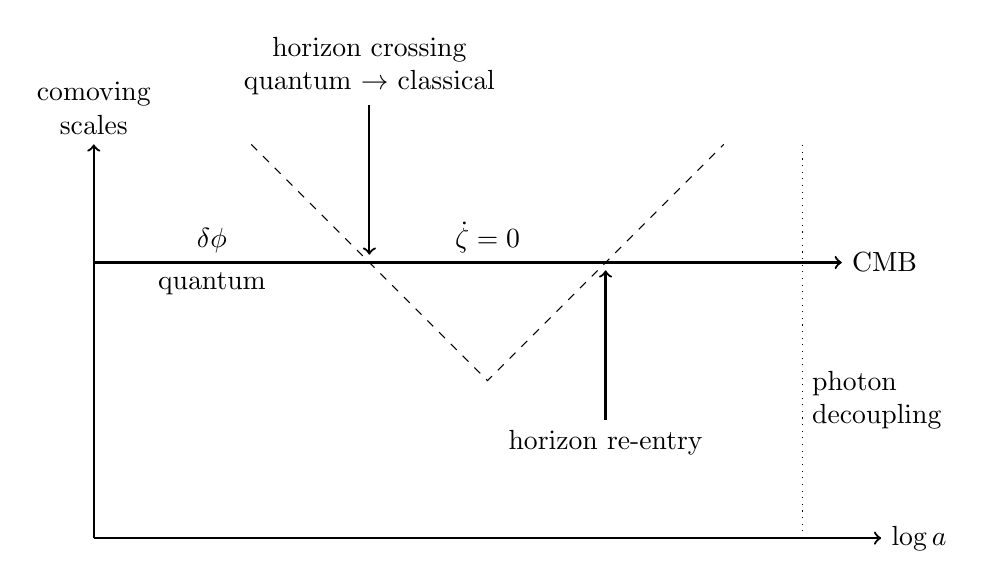
\begin{tikzpicture}
        \draw[thick,->] (0,0) -- (10,0) node[right] {\(\log a\)};
        \draw[thick,->] (0,0) -- (0,5) node[above,align=center] {comoving\\scales};
        \draw[dashed] (2,5) -- (5,2) -- (8,5);
        \draw[thick,->] (0,3.5) -- (9.5,3.5) node[right] {CMB};
        \node[above] at (1.5,3.5) {\(\delta\phi\)};
        \node[below] at (1.5,3.5) {quantum};
        \draw[thick,<-] (3.5,3.6) -- (3.5,5.5) node[align=center,above] {horizon crossing\\quantum \(\to\) classical};
        \node[above] at (5,3.5) {\(\dot\zeta=0\)};
        \draw[thick,<-] (6.5,3.4) -- (6.5,1.5) node[below] {horizon re-entry};
        \draw[dotted] (9,0) -- (9,5);
        \node[right,align=left] at (9,1.75) {photon\\decoupling};
    \end{tikzpicture}
\end{figure}

Recall the definition of the gauge-invariant constant density curvature perturbation:
\begin{equation}
    \zeta = -C + \frac13\nabla^2E + \mathcal{H}\frac{\delta\rho}{\bar\rho'}
\end{equation}
In the spatially flat gauge (\(C=E=0\)), this is just 
\begin{equation}
    \mathcal{H}\frac{\delta\rho}{\bar\rho'} = \mathcal{H}\delta\tau(\vb{x}) = \delta N_e(\vb{x}).
\end{equation}
During inflation, we have \(\delta\tau(\vb{x}) = \frac{\delta\phi}{\bar\phi'}\), so \(\zeta = \mathcal{H}\frac{\delta\phi}{\bar\phi'}\), and therefore the power spectrum is
\begin{equation}
    \Delta^2_\zeta(k) = \left(\frac{\mathcal{H}}{\bar\phi'}\right)\Delta^2_{\delta\phi}(k).
\end{equation}
Using \(\epsilon = \frac{\bar\phi^{'2}}{\mathcal{H}^2M_{\text{pl}}^2}\) and substituting in the \(\delta\phi\) power spectrum obtained above, we have
\begin{equation}
    \Delta^2_{\zeta}(k) = \frac1{8\pi^2\epsilon}\left(\frac{H}{M_{\text{pl}}}\right) \equiv A_s\left(\frac{k}{k_*}\right)^{n_s-1}.
\end{equation}
Approximate values (from COBE) are an amplitude of \(A_s = \SI{2.2e-9}{}\) and a spectral index of \(n_s = 0.96\pm0.01\).

Since \(H\) and \(\epsilon\) depend on time, we expect a small scale dependence i.e.\ deviation of \(n_s\) from 1. We have
\begin{equation}
    n_s - 1 = \dv{\log\Delta^2_\zeta(k)}{\log k} = \dv{\log\Delta^2_\zeta(k)}{N_e} \dd{N_e}{\log k}.
\end{equation}
Now
\begin{equation}
    \dv{\log\Delta^2_\zeta}{N_e} = -\dv{\log\epsilon}{N_e} + 2\dv{\log H}{N_e} = -\eta - 2\epsilon
\end{equation}
and
\begin{equation}
    \dv{\log k}{N_e} = \dv{\log(aH)}{N_e} = 1 + \dv{\log H}{N_e} = 1 + \epsilon,
\end{equation}
so we have
\begin{equation}
    n_s - 1 = \frac{-\eta-2\epsilon}{1+\epsilon} \approx -\eta-2\epsilon.
\end{equation}
Note that for \(|\eta|\ll 1\), we always obtain a red spectrum.

\subsection{From \texorpdfstring{$\zeta$}{zeta} to anisotropies of the CMB}

Typically our route is \(\zeta \to \delta\rho \to \Delta T_{\text{CMB}}(\vb{n}) \to C_l\). \(\Delta_T\) are anisotropies in the CMB which we decompose into spherical harmonics as
\begin{equation}
    \frac{\Delta T(\vb{n})}{T} = \sum a_{lm}Y_{lm}(\vb{n}).
\end{equation}
We then obtain angular power spectra as 
\begin{equation}
    C_l^{TT} = \frac1{2l+1}\sum_m\langle a^*_{lm}a_{lm}\rangle.
\end{equation}
We can write
\begin{equation}
    a_{lm} = 4\pi (-i)^l \int\frac{\dd[3]{k}}{(2\pi)^3} \Delta_{Tl}(k)\zeta_{\vb{k}}Y_{lm}(\vb{k}),
\end{equation}
which defines \(\Delta_{Tl}(k)\), the ``temperature transfer function''. Typically this is computed using some Boltzmann code such as \texttt{CMBFast} or \texttt{CAMB}. Then we have
\begin{equation}
    C_l^{TT} = \frac2\pi\int\dd{k}k^2\Delta^2_\zeta(k) \Delta_{Tl}^2(k).
\end{equation}

\subsection{Tensor perturbations}
Tensor perturbations provide robust and model-independent predictions of inflation. We observe tensor perturbations in the form of gravitational waves.

Consider a tensor perturbation to the metric. We have
\begin{equation}
    \dd{s}^2 = a^2(\tau)\left(-\dd{\tau}^2 + \left(\delta_{ij}+2\hat{E}_{ij}\right)\dd{x^i}\dd{x^j}\right),
\end{equation}
where \(\hat{E}_{ij}\) is traceless and conserved. Consider modes with \(\vb{k} = k\vb{z}\); we can write
\begin{equation}
    \frac{M_{\text{pl}}^2}{2}\hat{E}_{ij} = \frac1{\sqrt{2}}
    \begin{pmatrix}
        h_+ & h_\times & 0 \\
        h_\times & -h_+ & 0 \\
        0 & 0 & 0
    \end{pmatrix}.
\end{equation}
Varying \(h_+\) and \(h_-\) in the Einstein-Hilbert action leads to 
\begin{equation}
    h_\alpha'' + 2\mathcal{H}h_\alpha' + k^2h_\alpha = 0,\quad \alpha \in \{+,\times\}.
\end{equation}
Note that this equation is identical to that of the scalar perturbation. Therefore we have
\begin{align}
    \Delta^2_t(k) &= 2 \Delta^2_E \quad \text{(since we have two modes \(+,\times\))}\\
                  &= 2 \left(\frac2{M_{\text{pl}}}\right)^2\Delta^2_{\delta\phi}(k) \quad \text{(from Einstein equations)} \\
                  &= \frac8{M_{\text{pl}}^2}\left(\frac{H}{2\pi}\right)^2 
                  = \frac2{\pi^2}\left(\frac{H}{M_{\text{pl}}}\right)^2 
                  \equiv A_t \left(\frac{k}{k_*}\right)^{n_t-1}.
\end{align}
We have
\begin{equation}
    n_t - 1 = \dv{\log\Delta_t^2}{\log k} = \dv{\log H^2}{\log k} = \dv{\log H^2}{N_e}\dv{N_e}{\log k} \approx - 2\epsilon.
\end{equation}

A relevant observable is the \emph{tensor-to-scalar ratio}:
\begin{equation}
    r = \frac{A_t}{A_s} = \frac2{\pi^2}\left(\frac{H}{M_{\text{pl}}}\right)^2\cdot8\pi^2\epsilon\left(\frac{M_{\text{pl}}}{H}\right)^2 \cdot \underbrace{k^\eta}_{\mathclap{\approx1}} \approx 16\epsilon.
\end{equation}

\end{document}
